\documentclass[8pt,red]{beamer}
\usepackage{amsmath,amsthm,amsfonts,amssymb,amsbsy}
\everymath{\displaystyle}
\usepackage{stmaryrd} 
\usepackage{subeqnarray}

\usepackage{cases}
\usepackage{array}
\usepackage{pifont}

\usepackage{fancyhdr}

\makeatletter
  \def\Hy@PageAnchorSlidesPlain{}%
  \def\Hy@PageAnchorSlide{}%
\makeatother


\usepackage{lastpage}
\usepackage{subfig}
\usepackage{float}

\usepackage{graphicx}
\usepackage{subfloat}
\usepackage{rotating}
\usepackage{tikz}

\usetikzlibrary{arrows}
\usetikzlibrary{calc}


% \usepackage{algorithm}
% \usepackage{algorithmic}


\usepackage{minted}
\usepackage{color}



%% Symbole de fraction
\newcommand{\Frac}[2]{{\displaystyle \frac{\displaystyle #1}{\displaystyle #2}}}
\newcommand{\Prac}[2]{\displaystyle \genfrac{(}{)}{}{}{\displaystyle #1}{\displaystyle #2}}
\newcommand{\Crac}[2]{\displaystyle \genfrac{[}{]}{}{}{\displaystyle #1}{\displaystyle #2}}

\newcommand{\norme}[1]{\|#1\|}


\newcommand{\HRule}{\rule{\linewidth}{1mm}}

% Fonction mathématiques

\newcommand{\transposee}[1]{{\vphantom{#1}}^{\text{\tiny{\textsf T}}}{#1}}
%\newcommand{\argmin}{\mathop{\mathrm{argmin}}}
\newcommand{\argminn}{\mathop{\mathrm{argmin}}}
\newcommand{\lexicomin}{\mathop{\mathrm{lexicomin}}}
%\newcommand{\arg}{\mathop{\mathrm{arg}}}



\DeclareMathOperator{\rot}{rot}
\DeclareMathOperator{\sh}{sh}
\DeclareMathOperator{\ch}{ch}
%\DeclareMathOperator{\th}{th}
\DeclareMathOperator{\arcsh}{arcsh}
\DeclareMathOperator{\argth}{argth}
\DeclareMathOperator{\sign}{sign}




%%The Principal Value Integral symbol
\def\Xint#1{\mathchoice
   {\XXint\displaystyle\textstyle{#1}}%
   {\XXint\textstyle\scriptstyle{#1}}%
   {\XXint\scriptstyle\scriptscriptstyle{#1}}%
   {\XXint\scriptscriptstyle\scriptscriptstyle{#1}}%
   \!\int}
\def\XXint#1#2#3{{\setbox0=\hbox{$#1{#2#3}{\int}$}
     \vcenter{\hbox{$#2#3$}}\kern-.5\wd0}}
\def\ddashint{\Xint=}
\def\dashint{\Xint-}



% macro pour les symbols d'ensemble
%\nbOne
\def\nbOne{{\mathchoice{\rm 1\mskip-4mu l}{\rm 1\mskip-4mu l} {\rm 1 \mskip-4.5mu l}{\rm 1\mskip-5mu l}}}
%
%%  Les ensembles de nombres  C. Fiorio (fiorio.at.math.tu-berlin.de) 
%
\def\nbR{\ensuremath{\mathrm{I\!R}}} % IR
\def\nbN{\ensuremath{\mathrm{I\!N}}} % IN
\def\nbF{\ensuremath{\mathrm{I\!F}}} % IF
\def\nbH{\ensuremath{\mathrm{I\!H}}} % IH
\def\nbK{\ensuremath{\mathrm{I\!K}}} % IK
\def\nbL{\ensuremath{\mathrm{I\!L}}} % IL
\def\nbM{\ensuremath{\mathrm{I\!M}}} % IM
\def\nbP{\ensuremath{\mathrm{I\!P}}} % IP
%
% \nbOne : 1I : symbol one
\def\nbOne{{\mathchoice {\rm 1\mskip-4mu l} {\rm 1\mskip-4mu l}
{\rm 1\mskip-4.5mu l} {\rm 1\mskip-5mu l}}}
%
% \nbC   :  Nombres Complexes
\def\nbC{{\mathchoice {\setbox0=\hbox{$\displaystyle\rm C$}%
\hbox{\hbox to0pt{\kern0.4\wd0\vrule height0.9\ht0\hss}\box0}}
{\setbox0=\hbox{$\textstyle\rm C$}\hbox{\hbox
to0pt{\kern0.4\wd0\vrule height0.9\ht0\hss}\box0}}
{\setbox0=\hbox{$\scriptstyle\rm C$}\hbox{\hbox
to0pt{\kern0.4\wd0\vrule height0.9\ht0\hss}\box0}}
{\setbox0=\hbox{$\scriptscriptstyle\rm C$}\hbox{\hbox
to0pt{\kern0.4\wd0\vrule height0.9\ht0\hss}\box0}}}}
%
% \nbQ   : Nombres Rationnels Q
\def\nbQ{{\mathchoice {\setbox0=\hbox{$\displaystyle\rm
Q$}\hbox{\raise
0.15\ht0\hbox to0pt{\kern0.4\wd0\vrule height0.8\ht0\hss}\box0}}
{\setbox0=\hbox{$\textstyle\rm Q$}\hbox{\raise
0.15\ht0\hbox to0pt{\kern0.4\wd0\vrule height0.8\ht0\hss}\box0}}
{\setbox0=\hbox{$\scriptstyle\rm Q$}\hbox{\raise
0.15\ht0\hbox to0pt{\kern0.4\wd0\vrule height0.7\ht0\hss}\box0}}
{\setbox0=\hbox{$\scriptscriptstyle\rm Q$}\hbox{\raise
0.15\ht0\hbox to0pt{\kern0.4\wd0\vrule height0.7\ht0\hss}\box0}}}}
%
% \nbT   : T
\def\nbT{{\mathchoice {\setbox0=\hbox{$\displaystyle\rm
T$}\hbox{\hbox to0pt{\kern0.3\wd0\vrule height0.9\ht0\hss}\box0}}
{\setbox0=\hbox{$\textstyle\rm T$}\hbox{\hbox
to0pt{\kern0.3\wd0\vrule height0.9\ht0\hss}\box0}}
{\setbox0=\hbox{$\scriptstyle\rm T$}\hbox{\hbox
to0pt{\kern0.3\wd0\vrule height0.9\ht0\hss}\box0}}
{\setbox0=\hbox{$\scriptscriptstyle\rm T$}\hbox{\hbox
to0pt{\kern0.3\wd0\vrule height0.9\ht0\hss}\box0}}}}
%
% \nbS   : S
\def\nbS{{\mathchoice
{\setbox0=\hbox{$\displaystyle     \rm S$}\hbox{\raise0.5\ht0%
\hbox to0pt{\kern0.35\wd0\vrule height0.45\ht0\hss}\hbox
to0pt{\kern0.55\wd0\vrule height0.5\ht0\hss}\box0}}
{\setbox0=\hbox{$\textstyle        \rm S$}\hbox{\raise0.5\ht0%
\hbox to0pt{\kern0.35\wd0\vrule height0.45\ht0\hss}\hbox
to0pt{\kern0.55\wd0\vrule height0.5\ht0\hss}\box0}}
{\setbox0=\hbox{$\scriptstyle      \rm S$}\hbox{\raise0.5\ht0%
\hboxto0pt{\kern0.35\wd0\vrule height0.45\ht0\hss}\raise0.05\ht0%
\hbox to0pt{\kern0.5\wd0\vrule height0.45\ht0\hss}\box0}}
{\setbox0=\hbox{$\scriptscriptstyle\rm S$}\hbox{\raise0.5\ht0%
\hboxto0pt{\kern0.4\wd0\vrule height0.45\ht0\hss}\raise0.05\ht0%
\hbox to0pt{\kern0.55\wd0\vrule height0.45\ht0\hss}\box0}}}}
%
% \nbZ   : Entiers Relatifs Z
\def\nbZ{{\mathchoice {\hbox{$\sf\textstyle Z\kern-0.4em Z$}}
{\hbox{$\sf\textstyle Z\kern-0.4em Z$}}
{\hbox{$\sf\scriptstyle Z\kern-0.3em Z$}}
{\hbox{$\sf\scriptscriptstyle Z\kern-0.2em Z$}}}}
%%%% fin macro %%%%



\newcommand{\putidx}[1]{\index{#1}\textit{#1}}



\newcommand{\reffig}[1]{({\it cf} figure : \ref{#1})}
\newcommand{\refann}[1]{({\it cf} Annexe : \ref{#1})}


%\definecolor{darkgray}{gray}{.25}
\definecolor{gray}{gray}{.5}
\definecolor{lightgray}{gray}{.75}
%\definecolor{gradbegin}{rgb}{0,1,1}
%\definecolor{gradend}{rgb}{0,.1,.95}
%\newcommand{\newtexte}[1]{\textcolor{darkgray} {#1}}
\newcommand{\newtexte}[1]{{#1}}% macro pour les varibales favorites
% normal tangent
\def\n{{\hbox{\tiny{N}}}}
\def\t{{\hbox{\tiny{T}}}}
\def\ss{{\hbox{\tiny{S}}}}
\def\nt{\hbox{\tiny{NT}}}
\def\nsf{\hbox{\tiny{\textsf N}}}
\def\tsf{\hbox{\tiny{\textsf T}}}
\def\sigman{\sigma_{\n}}
\def\sigmat{\sigma_{\t}}
\def\sigmant{\sigma_{\nt}}
\def\epsn{\epsilon_{\n}}
\def\epst{\epsilon_{\t}}
\def\epsnt{\epsilon_{\nt}}
\def\eps{\epsilon}
\def\veps{\varepsilon}
\def\sig{\sigma}
% \def\Rn{R_{\n}}
% \def\Rt{R_{\t}}
\def\cn{c_{\n}}
\def\Cn{C_{\n}}
\def\ct{c_{\t}}
\def\Ct{C_{\t}}
\def\un{u_{\n}}
\def\ut{\buu_{\t}}
\def\uut{u_{\t}}
\def\unc{u_{\n}^c}
\def\utc{\buu_{\t}^c}
\def\vn{v_{\n}}
\def\vt{v_{\t}}
\def\rr{\hbox{\tiny{\textsf R}}}
\def\irr{\hbox{\tiny{\textsf{IR}}}}
\def\rn{r_{\n}}
\def\rt{\brr_{\t}}
\def\rnc{r_{\n}^c}
\def\rtc{\brr_{\t}^c}
\def\trn{\Tilde{r}_{\n}}
\def\trt{\Tilde{\brr}_{\t}}
\def\tr{\Tilde{\brr}}
\def\tv{\Tilde{\bvv}}
\def\vn{v_{\n}}
\def\vt{\bvv_{\t}}
\def\adh{\mathsf{adh}}
\def\adj{\hbox{\tiny{\textsf{adj}}}}
\def\adjc{\hbox{\tiny{\textsf{adjC}}}}
\def\adja{\hbox{\tiny{\textsf{adjA}}}}
\def\cc{\hbox{\tiny{\textsf C}}}
\def\ca{\hbox{\tiny{\textsf A}}}

% domaines et frontieres
\def\om{\Omega}
\def\oma{\Omega^{\alpha}}
\def\omu{\Omega^1\cup \Omega^2}
\def\gc{\Gamma_c}
\def\omt{\omu \cup \gc}
% derivee partielle et gradient et divergence
\def\p{\partial}
\def\grad{\nabla}
\def\div{\mathop{\rm div}\nolimits}
%

%\DeclareTextSymbol{\deg}{T1}{6}
%\def\degre{\mathdegree}
%\newcommand{\degre}{\mathdegree}

\def\etc{\textit{etc}\ldots}
\newcommand{\mdegre}{\hbox{\text{\degre}}}

%\def\nscd{\textsf{\bfseries NSCD}}
%\def\nscd{\textsf{NSCD}}
\newcommand{\nscd}{\textsf{NSCD}}
%\Pisymbol{psy}{212} ou encore \Pisymbol{psy}{228}




%----------------------------------------------------------------------
%             Des chiffres avec des ronds autour
%----------------------------------------------------------------------
\def\nombrecercle#1{\def\taille{0.3}
                \put(0,0){#1}
                \put(0.08,0.08){\circle{\taille}}}



\def\ae#1{\stackrel{\mbox{\scriptsize a.e.}}{#1}}
%\def\argmin{\mathop{\rm argmin}}


\def\eqref#1{{\rm (\ref{#1})\/}}
\def\indicfon{\mathord{\rm i}}       %indicator function
\def\p{\mathord{\rm proj}}
\def\N{\mathord{\rm N}}
% \def\prosca#1#2{#1\cdot#2}
\def\prosca#1#2{\langle #1,#2\rangle}
\def\qedtext{\mbox{}\hfill$\Box$}
\def\qedmath{\eqno\Box}

\def\s{{$\mathcal{S}$}}
\def\somme{\mathop{\textstyle\sum}}
\def\somme{\mathop{\textstyle\sum}}
\def\submoins{_{\scriptscriptstyle-}}
\def\subplus{_{\scriptscriptstyle+}}
\def\T{\mathord{\rm T}}

%----------------------------------------------------------------------
%             Macro M Jean 
%----------------------------------------------------------------------

\def\Real{\mbox{I\hspace{-.15em}R}}
\def\Integer{\mbox{I\hspace{-.15em}N}}
\def\Bunit{\mbox{I\hspace{-.15em}B}}
\def\real{\mbox{\scriptsize I\hspace{-.15em}R}}
\def\bunit{\mbox{\scriptsize I\hspace{-.15em}B}}
\def\IL{\mbox{\scriptsize I\hspace{-.15em}L}}
\def\Indic{\mbox{\large $\psi$}}
\def\bfxi{\mbox{$\xi$ \hspace{-1.1em} $\xi$}}
%\def\bfXi{\mbox{$\Xi$ \hspace{-1.1em} $\Xi$}}
\def\RunR{\mathcal R}
\def\RunRN{\mathcal R_{N}}
\def\RunRT{\mathcal R_{T}}
\def\RunS{\mathcal S}
\def\RunSN{\mathcal S_{N}}
\def\RunST{\mathcal S_{T}}
\def\RunU{\mathcal U}
\def\RunUN{\mathcal U_{N}}
\def\RunUT{\mathcal U_{T}}
\def\RunUP{\mathcal U'}
\def\RunUPN{\mathcal U'_{N}}
\def\RunUPT{\mathcal U'_{T}}
\def\RunJ{\mathcal J}
\def\RunW{\mathcal W}
\def\RunF{f}
\def\RunFa{f_{1}}
\def\RunFb{f_{2}}
\def\RunFP{f'}
\def\RunV{v}
\def\RunVP{v'}
\def\EspF{\mathcal F}
\def\EspV{\mathcal V}

\def\N{\mbox{I\hspace{ -.15em}N}}
\def\Z{\mbox{Z\hspace{ -.3em}Z}}
\def\Q{\mbox{l\hspace{ -.47em}Q}}
\def\R{\mbox{l\hspace{ -.15em}R}}
\def\F{\mbox{l\hspace{ -.15em}F}}
\def\E{\mbox{l\hspace{ -.15em}E}}
\def\LMGC90{{\small \it LMGC90 }}
\def\NSCD{{\small \it NSCD }}
\def\CHIC{{\small \it CHIC }}
\def\half{{\frac{_{1}}{^{2}}}}
\def\12T{{\frac{_{1}}{^{2T}}}}

\def\geq{\geqslant}
\def\leq{\leqslant}
\def\ge{\geqslant}
\def\le{\leqslant}


\begingroup
\count0=\time \divide\count0by60 % Hour
\count2=\count0 \multiply\count2by-60 \advance\count2by\time
% Min
\def\2#1{\ifnum#1<10 0\fi\the#1}
\xdef\isodayandtime{\the\year-\2\month-\2\day\space\2{\count0}:%
\2{\count2}}
\endgroup

%---------------------------------------------------------------------
%             Redaction note environnement B. Brogliato
%----------------------------------------------------------------------
\makeatletter

{\newtheorem{ndr1bb}{\textbf{\textsc{Redaction note B.B.}}}[section]}

\newenvironment{ndrbb}%
{%
\noindent\begin{ndr1bb}\hrule\vspace{1em}%
\ttfamily\small
}%
{%
\begin{flushright}%
%\vspace{-1.5em}\ding{111}
\end{flushright}%
\vspace{-1.5em}\hrule
\end{ndr1bb}%
}
%----------------------------------------------------------------------
%             Redaction note environnement V.ACARY
%----------------------------------------------------------------------
% Faut etre fou pour s'amuser a pondre des notes pareilles

{\newtheorem{ndr1va}{\textbf{\textsc{\footnotesize Redaction note V.A.}}}[section]}

\newenvironment{ndrva}%
{%
\noindent\begin{ndr1va}\hrule\vspace{1em}%
\ttfamily\small \  \\
\noindent}%
{%
$ $ \\
\hrule
\end{ndr1va}%
}
\makeatother








% ----------------DEFINITIONS-----------------
% 

 \def\II{\mathop{{\rm I}\mskip-3.0mu{\rm I}}\nolimits}




% -----------------------------------
 \def\c{\mathop{{\rm 1}\mskip-10.0mu{\rm C}}\nolimits}
 \def\C{\mathop{{\rm 1}\mskip-10.0mu{\rm C}}\nolimits}
 \def\ZZ{\mathaccent23Z}
% 

\newcommand{\ie}{{\textit{i.e.}}}


%\def\sgn{\mbox{\rm sgn}}
\DeclareMathOperator{\sgn}{sgn}
\DeclareMathOperator{\proj}{proj}
\DeclareMathOperator{\prox}{prox}
\DeclareMathOperator{\argmin}{argmin}

\newcommand{\RR}{\mbox{\rm $I\!\!R$}}
\newcommand{\NN}{\mbox{\rm $I\!\!N$}}


% ---------------- MMC -----------------
% 

\newcommand{\contract}{{\,:\,}}

\newcommand{\scontract}{{\,{\Bar\otimes}\,}}
\newcommand{\tcontract}{{\,{\Bar{\Bar{\Bar\otimes}}}\,}}


\newcommand{\DP}[2]{\displaystyle \frac{\partial {#1}}{\partial {#2}}}

% %\newtheorem{definition}{Definition}
% \newtheorem{proposition}{Proposition}
% \newtheorem{lemma}{Lemma}

% \newtheorem{claim}{Claim}
% \newtheorem{remark}{Remark}
% \newtheorem{assumption}{Assumption}
% \newtheorem{example}{Example}
% \newtheorem{conjecture}{Conjecture}
% \newtheorem{corollary}{Corollary}
% \newtheorem{OP}{OP}
% \newtheorem{problem}{Problem}
% \newtheorem{theorem}{Theorem}


\def\dt{{\rm d}t}
\def\dv{{\rm d}v}
\def\di{{\rm d}i}
\def\dI{{\rm d}I}
\def\dU{{\rm d}U}


\def\nat{{\hbox{\tiny{nat}}}}
\def\nor{{\hbox{\tiny{nor}}}}
\def\fb{\hbox{\tiny{\textsf FB}}}
\def\vione{{\hbox{\tiny{vi-1}}}}
\def\vitwo{{\hbox{\tiny{vi-2}}}}
\def\qvitwo{{\hbox{\tiny{qvi-2}}}}
\def\acone{{\hbox{\tiny{ac-1}}}}
\def\actwo{{\hbox{\tiny{ac-2}}}}


\usepackage{wasysym}

\makeatletter
\newcommand{\pushright}[1]{\ifmeasuring@#1\else\omit\hfill$\displaystyle#1$\fi\ignorespaces}
\newcommand{\pushleft}[1]{\ifmeasuring@#1\else\omit$\displaystyle#1$\hfill\fi\ignorespaces}
\makeatother


\setbeamertemplate{theorem}[ams style]
\setbeamertemplate{theorems}[numbered]
\usepackage[backend=biber,style=authoryear,bibstyle=authoryear,citestyle=authoryear-comp,natbib=true,maxcitenames=2,uniquelist=false,uniquename=false,bibencoding=utf8]{biblatex}
\addbibresource{./biblio/String.bib}
\addbibresource{./biblio/NonSmooth.bib}
\addbibresource{./biblio/Math.bib}
\addbibresource{./biblio/Multibody.bib}
\addbibresource{./biblio/Fem.bib}
\addbibresource{./biblio/Dae.bib}
\addbibresource{./biblio/Meca.bib}
\addbibresource{./biblio/AnaNum.bib}
\addbibresource{./biblio/Math-Impact.bib}
\addbibresource{./biblio/Contact.bib}
\addbibresource{./biblio/Optim.bib}
\addbibresource{./biblio/Cp.bib}

% %hideothersubsections
% \usetheme[hideothersubsections,width=2.5cm]{Goettingen}
% %\useoutertheme[headline=empty]{miniframes}

\usetheme[]{Montpellier}
\makeatletter
\useoutertheme[height=0pt, width=0cm]{sidebar}
{\usebeamercolor{structure}}
\setbeamertemplate{sidebar canvas \beamer@sidebarside}[vertical shading][top=structure.fg!25,bottom=structure.fg!10]

%%% Local Variables: 
%%% mode: latex
%%% TeX-master: t
%%% End: 


% \title{Formulations and extensive comparisons of 3D frictional contact solvers based on performance profiles}
% \author{Vincent Acary, Maurice Br\'emond, Olivier Huber \\ INRIA Rh\^one--Alpes, Grenoble.}
% \date{CMIS 2018, Biella, Italy}


\title[Siconos/numerics and FCLIB]{Siconos/numerics and FCLIB: a collection of solvers and benchmarks for solving frictional contact problems \\[5mm]
  \large{CMIS,  May 2024}}

\author{Vincent Acary}
\date{
   \includegraphics[height=0.15\textheight]{./logos/inr_logo_rouge.jpg}\hfill
   \includegraphics[height=0.15\textheight]{./logos/logo_ljk2.pdf}\hfill
   \includegraphics[height=0.15\textheight]{./logos/logo_uga_transparent.png}\\
  
 }
 \institute{Inria -  Centre de l'Université Grenoble Alpes - Laboratoire Jean Kuntzmann}


\setbeamertemplate 
{footline} 
{\quad\hfill\strut\insertsection\quad--\quad\insertframenumber/\inserttotalframenumber\strut\quad\quad} 

\graphicspath{{../figure/}}

% \includeonly{%
% %  introduction,
%   fc3d,
%   existence,
%   numerics,
%   comparison
% }



%\newtheorem{defn}{Definition}
%\renewcommand{\thedefn}{\arabic{defn}}
% \newtheorem{thm}[defn]{Theorem}
% \newtheorem{corr}[defn]{Corollary}
% \newtheorem{ass}[defn]{Assumption}
% \newtheorem{lem}[defn]{Lemma}
% \newtheorem{rem}[defn]{Remark}
% \newtheorem{hypo}[defn]{Hypotheses}
% \newtheorem{exmp}[defn]{Example}
% \newtheorem{prop}[defn]{Proposition}
\newcommand{\diag}{\mbox{\rm diag}}
\newcommand{\co}{\overline{\mathit{co}}}
\newcommand{\rect}{\overline{\mathit{rect}}}
\newcommand{\newb}{g}

\renewcommand{\tr}[1]{\textcolor{red}{#1}}




\begin{document}


\frame{\titlepage
}


%\section{Introduction}

% \begin{frame}
% %  \frametitle{Introduction. Bio.}
%   \begin{block}
%     {Team-Project TRIPOP.\\ INRIA. Centre de recherche de l'Université Grenoble Alpes (UGA)}
%     ``Jean Jacques Moreau's fan club''. Convex Analysis and Nonsmooth Mechanics.
%     \begin{itemize}
%     %\item Scientific leader :  Bernard Brogliato
%     \item $6$ permanents, $6$ PhD, $4$ Post-docs, $3$ Engineer,
%     \item Nonsmooth simulation and numerical modeling for natural gravitational risk in mountains.
%     \item Nonsmooth dynamical systems :
%       Modeling, analysis, simulation and Control.
%     \end{itemize}
%   \end{block}
%     \begin{block}
%       {Current Personal research themes}
%     \begin{itemize}
%     \item Nonsmooth Dynamical systems in the large:\\
%       Higher order Moreau's sweeping process. Complementarity systems and Filippov systems
%     \item Time--integration techniques for nonsmooth mechanical systems:\\ Mixed higher order schemes, Time--discontinuous Galerkin methods, Projected time--stepping schemes and generalized $\alpha$--schemes.
%     %\item Modeling and simulation of switched electrical circuits
%     %\item Discretization method for sliding mode control and Optimal control.
%     \item Formulation and numerical solvers for Coulomb's friction and Signorini's problem.% Second order cone programming.
%     \item Non-associated plasticity of geomaterials with contact, friction and impact
%     \item Coupling SPH/DEM/FEM and MPM/DEM/FEM
%     \item Data-driven modeling and data assimilation.
%     \end{itemize}
%   \end{block}
% \end{frame}



\frame{\tableofcontents}


%\include{introduction}
%\frame{\tableofcontents}


\section{The discrete frictional contact problem}
\label{Sec:fc3d}

\subsection{Signorini condition and Coulomb's friction}

\frame{
  \frametitle{Signorini's condition and Coulomb's friction} 
  \begin{minipage}[c]{0.45\linewidth}
    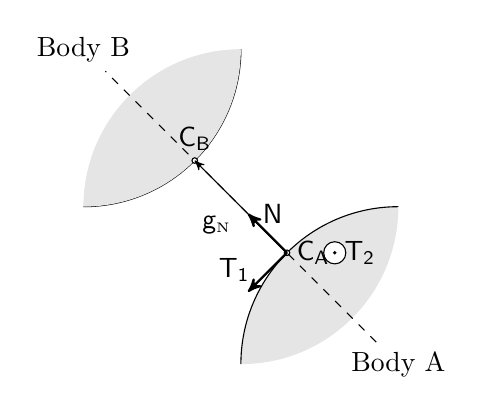
\begin{tikzpicture}[ scale=2,
      axis/.style={ ->, >=stealth'},
      normal/.style={ thick, ->, >=stealth'},
      important line/.style={very thick}, 
      dashed line/.style={dashed, thin},
      every node/.style={color=black},
      soldot/.style={only marks,mark=*},
      holdot/.style={fill=white,only marks,mark=*}
      ]
      % body
      \node (BodyA) at (1,-1) {Body A};
      \fill[gray!20] (1,0) arc (0:-90:1);
      \fill[gray!20] (1,0) arc (90:180:1);
      \draw (1,0) arc (90:180:1);

      \node (BodyB) at (-1,1) {Body B};
      \draw (0,1) arc (0:-90:1);
      \fill[gray!20] (0,1) arc (90:180:1);
      \fill[gray!20] (0,1) arc (0:-90:1);

      % local frame
      \def\nlength{0.35};
      \coordinate (CA)  at  ({1.0-sqrt(2)/2.0},{-1.0+sqrt(2)/2.0});
      \node[] at  (CA) [right] {$\sf C_A$};
      \draw[holdot]  (CA) circle(0.05em);
      \draw[normal] (CA) -- ($(CA)+({-\nlength*sqrt(2)/2.0},{+\nlength*sqrt(2)/2.0 })$) node [right] {$\,\sf N$};
      \draw[normal] (CA) -- ($(CA)+({-\nlength*sqrt(2)/2.0},{-\nlength*sqrt(2)/2.0 })$) node [above] {$\sf T_1\quad$};
      \draw[dashed line] (BodyA) -- (BodyB);
      \draw[holdot] ($(CA)+({\nlength*sqrt(3)/2.0},{0.0})$) circle(0.2em);
      \node at ($(CA)+({\nlength*sqrt(3)/2.0},{0.0})$) [right]{$\sf T_2$};
      \draw[soldot] ($(CA)+({\nlength*sqrt(3)/2.0},{0.0})$) circle(0.02em);
      
      \coordinate (CB)  at  ({-1.0+sqrt(2)/2.0},{1.0-sqrt(2)/2.0});
      \node at  (CB) [above] {$\sf C_B$};
      \draw[holdot]  (CB) circle(0.05em);

      \draw[axis] (CA) -- (CB) node[midway, below left ] {$\sf g_\n$} ;

      % \draw[axis] (0,-0.4) -- (0,0.4) node(yline)[right] {$\sgn(x)$};
      % % lines
      % \draw[important line] (-0.4,-0.3) -- (0.   ,-.3);
      % \draw[important line] (0.0,0.3) --(.4,.3)  ;
      % \coordinate (O) at (0.0, 0.05);
      % \draw[fill] (O) circle (0.03em);
      % \draw (0.0,0.05) node[right]{$a$};
      % \draw (0.0,0.3) node[left]{$1$};
      % \draw (0.0,-0.3) node[right]{$-1$};
      % \draw[holdot] (0.0,0.3) circle (0.03em);
      % \draw[holdot] (0.0,-.3) circle (0.03em);
    \end{tikzpicture}
  \end{minipage}
\begin{minipage}[c]{0.49\linewidth}
    \begin{itemize}
    \item gap function $ g_{\n} = (C_B-C_A) \sf N.$
    \item reaction forces and  velocities
      $$r =  r_\n {\sf N} + r_\t, \quad \text{ with  } r_\n \in \nbR, \quad r_\t \in \nbR^2.$$
      $$u =  u_\n {\sf N} + u_\t, \quad \text{ with } u_\n \in \nbR \quad u_\t \in \nbR^2.$$
    \item Signorini conditions
      $$  \text{ position level : }  0 \leq g_{\n} \perp r_\n \geq 0.$$\\
      $$ \text{velocity level : }\left\{\begin{array}{ll}
            0 \leq u_{\n} \perp r_\n \geq 0  &\text{ if } g_{\n} \leq 0\\
            r_{\n} =0 &\text{ otherwise}.
          \end{array}\right.$$
    \end{itemize}

  \end{minipage}
}
\frame{
  \frametitle{Signorini's condition and Coulomb's friction} 
  \begin{block}{Coulomb friction modeling assumption}
   Let $\mu$ be the coefficient of friction.  Let us define the Coulomb friction cone $K$ which is chosen as the
    isotropic second order cone
    \begin{equation}
      \label{eq:CoulombCone}
      K = \{r \in \nbR^3 \mid \|r_\t\| \leq \mu r_\n\}.
    \end{equation}
    Coulomb friction postulates
    \begin{itemize}
    \item for the \tr{sticking case} that
      \begin{equation}
        \label{eq:Coulom-stick}
        u_{\t} =0,\quad r \in K,
      \end{equation}
    \item and for the \tr{sliding case} that
      \begin{equation}
        \label{eq:Coulom-slide}
        u_{\t}  \neq 0,\quad \|r_\t\| = \mu r_\n , \quad  r_\t = - \frac{u_\t}{\|u_\t\|}\|r_\t\|.
      \end{equation}
    \end{itemize}
  \end{block}

  \begin{block}
    {Disjunctive formulation of the frictional contact behavior}
    \begin{equation}
      \label{eq:contact-disjunctive}
      \left\{\begin{array}{llr}
          r = 0  &\text{ if } g_{\n} > 0  & \text{(no contact)}\\
          r = 0,  u_\n \geq 0   &\text{ if } g_{\n} \leq 0 & \text{(take--off)} \\
          r \in K, u =0 &\text{ if } g_{\n} \leq 0 & \text{(sticking)}  \\
               r \in \partial K,u _\n=0, {r_\t} = - \frac{u_\t}{\|u_\t\|}\|r_\t\|  &\text{ if } g_{\n} \leq 0 & \text{(sliding)}  \\
        \end{array}\right.
    \end{equation}
  \end{block}
  

}

\frame{
  \frametitle{Signorini's condition and Coulomb's friction} 
  
  \begin{block}{Second Order Cone Complementarity (SOCCP) formulation}
  
    \begin{itemize}
    \item Modified relative velocity $\tilde u \in \nbR^3$ \citep{DeSaxce92} defined by 
      \begin{equation}
        \label{eq:modified-velocity}
        \tilde u = u +\mu \|u_\t\| \sf N.
      \end{equation}
    
    \item  Second-Order Cone Complementarity Problem (SOCCP) 
      \begin{equation}
        \label{eq:contact-SOCCP}
        K^\star \ni \tilde u \perp r \in K
      \end{equation}
      if $ g_\n \leq 0 $ and $r=0$ otherwise.\\[1mm]
      The set $ K^\star $ is
      the dual convex cone to $K$ defined by
      \begin{equation}
        \label{eq:dual-cone}
        K^\star = \{u \in \nbR^3 \mid  r^\top u \geq 0, \quad \text{for all } r \in K   \}.
      \end{equation}

    \end{itemize}
 \end{block}
    \vfill \small
    \citep{Acary.Brogliato2008,Acary.ea_ZAMM2011}

}
\frame{
  \frametitle{Signorini's condition and Coulomb's friction} 
   \begin{figure}[htbp]
  \centering
  \resizebox{!}{0.8\textheight}{\input{../figure/cone1-b.pdf_t}}
  \caption{Coulomb's friction and the modified velocity $\tilde u$. The sliding case.}
  \label{fig:CoulombFrictionSlidingDeSaxce}
\end{figure} 
}

\subsection{Definition}


% \frame{
%   \frametitle{3D frictional contact problem} 
%   \begin{block}{Multiple contact notation}
%     For each contact $\alpha \in \{1,\ldots n_c\}$, we have
%     \begin{itemize}
%     \item the local velocity : $u^\alpha \in \nbR^3$, and
%       $$  u = [[u^\alpha]^\top, \alpha = 1\ldots n_c]^\top$$
%     \item the local  reaction vector $r^\alpha\in \nbR^3$    
%       $$  r = [[r^\alpha]^\top, \alpha = 1\ldots n_c]^\top$$
%     \item the local  Coulomb cone    $$K^{\alpha}  = \{r^\alpha, \|r^\alpha_\t \| \leq \mu^\alpha |r^\alpha_\n| \} \subset \nbR^3$$
%        and the set $K$ is the cartesian product of Coulomb's friction cone at each contact, that 
%       \begin{equation}
%         \label{eq:CC}
%         K = \prod_{\alpha=1\ldots n_c} K^{\alpha} 
%       \end{equation}
%       and $K^\star$ is dual.
%     \end{itemize} \end{block}
  
% }





\frame{
  \frametitle{Discrete frictional contact problems} 
  \begin{problem}[General discrete frictional contact problem]\label{prob:I}
  Given
  \begin{itemize}
    \item a symmetric positive definite matrix ${M} \in \nbR^{n \times n}$,
    \item a vector $ {f} \in \nbR^n$,
    \item a matrix  ${H} \in \nbR^{n \times m}$,
    \item a vector $w \in \nbR^{m}$,
    \item a vector of coefficients of friction $\mu \in \nbR^{n_c}$,
  \end{itemize}
find three vectors $ {v} \in \nbR^n$, $u\in\nbR^m$ and $r\in \nbR^m$, denoted by $\mathrm{FC/I}(M,H,f,w,\mu)$  such that
\begin{equation}\label{eq:soccp1}
  \begin{cases}
    M v = {H} {r} + {f} \\[2mm]
    u = H^\top v + w \\[2mm]
    \tilde u = u + g(u) \\[2mm]
    K^\star \ni {\tilde u} \perp r \in K
  \end{cases}
\end{equation}
with $g(u) = [[\mu^\alpha  \|u^\alpha_\t\| {\sf N}^\alpha]^\top, \alpha = 1\ldots n_c]^\top$. 
\qed
\end{problem}

}

\frame{
  \frametitle{Discrete frictional contact problems}
  \only<1>{ \begin{block}{Wide range of applications}
      The problem is:
      \begin{itemize}
      \item is generic enough to include a large number of cases in practice,
      \item is really representative in the linear, or the linearized,  case (Newton procedure),
      \item can be generalised to non-linear cases.
      \end{itemize}
  \end{block}
  See for instance~\parencite{Acary.Cadoux2013}\\
  
 
  \begin{block}{Origin of the linear relation $u = H^\top v + w$}

     \begin{itemize}
     \item $H$ is the contact configuration matrix (similar to the Jacobians of the constraints)
     \item $w$ can contain
       \begin{itemize}
       \item impact laws terms or prescribed velocity in velocity level formulations
       \item displacements, or increments of displacements, in position level formulations
       \end{itemize}
     \end{itemize}
   \end{block}
 }
}
\frame{
  \frametitle{Discrete frictional contact problems}
   \only<1>{
     \begin{block}{Origin of the linear relation $  M v = {H} {r} + {f}$}
       \begin{itemize}
    
       \item Time--discretization of the discrete dynamical mechanical
         system. Event--capturing or event--detecting  time--stepping schemes
       \item Space discretization of the quasi--static problem of solids (FEM)\\
         (M is the tangent stiffness matrix !).
       \item Time--discretization and space discretization of the
         dynamic problem of solids. (FEM, MPM, PFEM, \ldots)

       \item Flexible or rigid  multi-body Systems,
       \item Spectral methods, harmonic balance method, \ldots
       \end{itemize}
     \end{block}
    }
}
\frame{
  \frametitle{Discrete frictional contact problems} 
  \begin{problem}[Reduced discrete frictional contact problem]\label{prob:II}
    Given
    \begin{itemize}
    \item a symmetric positive semi--definite  matrix ${W} \in \nbR^{m \times m}$,
    \item a vector $ {q} \in \nbR^m$,
    \item a vector $\mu \in \nbR^{n_c}$ of coefficients of friction, 
    \end{itemize}
    find two vectors $u\in\nbR^m$ and $r\in \nbR^m$, denoted by $\mathrm{FC/II}(W,q,\mu)$  such that
    \begin{equation}\label{eq:soccp2}
      \begin{cases}
        u =Wr +q \\[2mm]
        \tilde u =u + g(u) \\[2mm]
        K^\star \ni {\tilde u} \perp r \in K
      \end{cases}
    \end{equation}
    with $g(u) = [[\mu^\alpha \|u^\alpha_\t\| {\sf N}^\alpha]^\top,  \alpha = 1\ldots n_c]^\top$.
    \qed
  \end{problem}
  
  \begin{block}{Relation with the general problem}
     $ W = H^\top M^{-1} H$ and $q = H^\top  M^{-1} f + w $.
  \end{block}
  
}
\subsection{From the optimization point of view}
\frame{
  \frametitle{From the optimization point of view} 
%  \begin{block}{Complementarity problem / Variational inequality}
    Discrete frictional contact are complementarity problems / variational inequalities. \\[3mm]
    \quad\tr{Finite dimensional Second-Order Cone Complementarity Problems (SOCCP)}
    \begin{equation}
      \label{eq:soccp3}
      K^\star \ni Wr +q + g(Wr +q) \perp r \in K
    \end{equation}
    of more generally,\\[1mm]
    \quad\tr{Variational Inequality (VI)} (normal cone inclusion)
    \begin{equation}
      \label{eq:inclusion-1}
      -(W r +q + g(Wr+q)) \stackrel{\Delta}= - F(r)  \in N_K(r).
    \end{equation}
%  \end{block}
  \begin{block}{Properties}
    \begin{itemize}
    \item nonsmooth since  $g()$ is nonsmooth
    \item nonmonotone since the mapping $F$ is not monotone for large $\mu$
    \item many possible reformulations such as nonsmooth equations $G(r) = 0$
    \end{itemize}
  \end{block}
}  
\frame{
  \frametitle{From the optimization point of view}

  \begin{block}{Important Remarks}
    \begin{itemize}
    \item The variational inequality is NOT  the optimality condition of a (convex) optimization problem.
    \item The problem is hard to solve efficiently and robustly at tight accuracy.
    \item Even harder if $H$ is not full rank (constraints redundancy) 
    \item Generic numerical methods for VI/CP exist and can be applied
    \item Numerous of existing methods for FC3D problems are adaptations of mathematical programming methods.
    \end{itemize}
  \end{block}
}
\frame{
  \frametitle{From the optimization point of view}
  \begin{block}{Semismooth Newton methods for nonsmooth equations $G(r) = 0$.}
    Not just adaptations, but sometimes pioneering methods.
    \begin{itemize}
    \item The natural map $F^\nat$ associated with the VI (\ref{eq:inclusion-1}) $$ F^\nat(r) = r - P_{K}(r-F(r))$$
    \item Pioneering work of~\cite{Alart.Curnier1991}
      \begin{equation*}
        \label{eq:CKPS-1}
        \begin{cases}
          r_\n - P_{\nbR^{n_c}_+}(r_\n - \rho_\n  u_\n) = 0, \\
          r_\t - P_{D(\mu, r_{\n,+}+\rho u_\n)}(r_\t - \rho_\t u_\t   )=0,
        \end{cases}
      \end{equation*}
     
    \item other SOCCP functions (Fisher-Bursmeister function)
      
    \end{itemize}
  \end{block}
  
 
 }
 \frame{
  \frametitle{From the optimization point of view} 
  \begin{block}{An optimization problem}

    \begin{equation}
      \label{eq:2}
      \begin{array}{lcl}
        \min_{v,u,r} & & \tilde u ^\top r = u^\top r + \mu r_\n \|u_{\t}\|  \stackrel{\Delta}= b(u,r)\\[1mm]
        \text{s.t.} & & Mv = H r + f \\[1mm]
                    & & \tilde u = H^\top v + w + g(u) \in K^\star \\[1mm]
                    & & r \in K 
        
      \end{array}
    \end{equation}
    $b(u,r)$ is the de Saxcé bi-potential.
    \begin{itemize}
    \item A solution of the discrete frictional contact problem is a solution of the optimization problem \eqref{eq:2} with $b(u,r)=0$
    \item A solution of the optimization problem \eqref{eq:2} is a solution of the discrete frictional contact problem if $b(u,r)=0$
    \item With constraints qualification, the problem has a solution.
    \item The problem is not convex and non smooth, may have a lot of local minima.
 
    \end{itemize}
    \ding{220} In practice,  finding a minimum is difficult, and a global minimum is not ensured.
   
  \end{block}

}
  

 


%%% Local Variables:
%%% mode: latex
%%% TeX-master: "s"
%%% End:

\frame{\tableofcontents}

% 
\section{An existence result}
\label{Sec:existence}

\frame{
  \frametitle{An existence result  via convex optimization}

  PhD of F. Cadoux with  C. Lemaréchal and J. Malick \citep{Cadoux2009,Acary.ea_ZAMM2011}\\[2mm]

  
  Let us introduce a slack variable
  \begin{equation*} \label{eq:chgVarDS}
    s^\alpha := \| u^\alpha_\t \|
  \end{equation*}
  New formulation of the modified velocity with $A \in \nbR^{m\times n_c}$
  $$ \tilde u := u + A s \quad\quad  (g(u) = A s)$$
  The problem $\mathrm{FC/I}(M,H,f,w,\mu)$ can be reformulated as
  \begin{equation}\label{eq:soccp1-convex}
  \begin{cases}
    M v = {H} {r} + {f} \\[2mm]
    \widetilde  u = H^\top v + w  + A s  \\[2mm]
    K^\star \ni {\tilde u} \perp r \in K
  \end{cases}
\end{equation}
with
\begin{equation}
  \label{eq:3}
  s^\alpha := \| u^\alpha_\t \|
\end{equation}

}
\frame{
  \frametitle{An existence result.}
  The problem~(\ref{eq:soccp1-convex}) appears to be the KKT condition of
  \begin{block}{Primal problem}
    \begin{equation} \tag{$D_s$}
      \left\{
        \begin{array}{l}
          \min \quad J(v) := \frac{1}{2} v^\top M v + f^\top v \\
          H^\top v + w + A s \in K^\star
        \end{array}
      \right.
    \end{equation}
  \end{block}
  \begin{block}{Dual problem}
    \begin{equation} \tag{$P_s$}
      \left\{
        \begin{array}{l}
          \min \quad J_s(r) := \frac{1}{2} r^\top W r - q_s^\top r \\
          r \in K
        \end{array}
      \right.
    \end{equation}
    with $q_s = q + A s $
  \end{block}
  \begin{block}{Interest}
    Two convex programs \ding{220} existence of solutions under feasibility conditions.
  \end{block}
}
\frame{
  \frametitle{An existence result.}
  \begin{block}{Fixed point problem}
    Introducing
  $$ u(s) := \argmin_u (P_s) = \argmin_u (D_s) $$
  practically \alert{computable} by optimization software, and
  $$ F^\alpha(s) := \| u^\alpha_T(s) \|, $$
  the incremental problem becomes a fixed point problem
  $$ F(s) = s $$
\end{block}

}
\frame{
  \frametitle{An existence result.}

  \begin{block}{Key assumption}
    \begin{equation}
      \exists v \in \R^m \ : \ H v + w \in {\rm int }K^\star \label{eq:key-assumption}
  \end{equation}
  \end{block}
  Using Assumption~(\ref{eq:key-assumption}),
  \begin{itemize}
  \item the application $F: \R_+^n \rightarrow \R_+^n$ is \alert{well-defined}, \alert{continuous} and \alert{bounded}
  \item apply Brouwer's theorem
  \end{itemize}
  \begin{theorem}
    A fixed point exists
  \end{theorem}
  %This result is a variant of a previous result obtained by~\cite{Klarbring.Pang1998}.
}
\frame{
  \frametitle{An existence result.}
  \begin{block}{Numerical validation of the key assumption}
    Solving a SOC linear program:  find $x^\star \in \RR$
    \begin{equation*}
      \label{eq:min-SOC}
      \begin{array}{lcl}
        \max_x & &  x \\
       \text{s.t.} & &  H v + w - a x \in K^\star
      \end{array}
    \end{equation*}
    where $a = \rm{col}(N^{\alpha}, \alpha \in \llbracket 1, m\rrbracket)\in \nbR^m$.\\
    If $x^\star > 0$, then the assumption is satisfied.
  \end{block}
  \begin{block}{Numerical interest}
    The fixed point equation $F(s) = s$ can be tackled by
    \begin{itemize}
    \item \alert{fixed-point} iterations
      $$ s \leftarrow F(s) $$
    \item \alert{Newton} iterations
      $$s \leftarrow \mathrm{Jac}[F](s) \backslash F(s) $$
    \end{itemize}
    The inner problem can be solved by QP  solvers with SOC constraints (ADMM, IPM, AL, \ldots... ) 
  \end{block}
}


%%% Local Variables: 
%%% mode: latex
%%% TeX-master: "s"
%%% End: 

% \frame{\tableofcontents}


\section{Numerical methods}
\label{Sec:Numerics}

\frame{
  \frametitle{Numerical solution procedure}
  \begin{itemize}
  \item VI based methods
  \item Nonsmooth Equations based methods
  \item Matrix block--splitting and projection based algorithms
  \item Proximal point algorithms
  \item Optimization based approach
  \item Interior point techniques
  \end{itemize}
}






\subsection{VI based methods}

\frame{
  \frametitle{VI based methods}
  \begin{block}{Standard methods}
    \begin{itemize}
    \item Basic fixed point iterations with projection\hfill\tr{\sf{[FP-VI]}}
      $$\sf z_{k+1} \leftarrow P_{X}(z_k - \rho_k\,F(z_k))$$
  \item Extragradient method\hfill\tr{\sf{[EG-VI]}}
    $$\sf z_{k+1} \leftarrow P_X(z_{k}-\rho_k\,F(P_X(z_k-\rho_k F(z_k))))$$
  \end{itemize}
\end{block}
With fixed $\rho$, we get the Uzawa Algorithm of De Saxc\'e-Feng\hfill\tr{\sf{[FP-DS]}}
\begin{block}
{Self-adaptive procedure for $\rho_k$}\hfill\tr{\sf{[UPK]}}
 \begin{equation*}
   \label{eq:Korpelevitch}
   \text{Armijo-like : } m_k\in \NN\quad  \text{such that }
   \left\{  \begin{array}{l}
              \rho_k = \rho 2^{m_k},\\[1mm]
              \rho_k \| F(z_k)-F(\bar z_k) \| \leq \|z_k-\bar z_k\|
            \end{array}\right.
 \end{equation*}
\end{block}

  
}


\subsection{Nonsmooth Equations based methods}
\frame{
  \frametitle{Nonsmooth Equations based methods}
  \only<1>
  {\begin{block}  {Nonsmooth Newton on $G(z)=0$}

   $$z_{k+1}  =  z_k -  \Phi^{-1}(z_k) (G(z_k)), \quad\quad\Phi(z_k) \in \partial G(z_k)$$
   \begin{itemize}
   \item Alart--Curnier Formulation~\citep{Alart.Curnier1991}\hfill\tr{\sf{[NSN-AC]}}
     \begin{equation*}
       \label{eq:CKPS-1}
       \begin{cases}
         r_\n - P_{\RR^{n_c}_+}(r_\n - \rho_\n  u_\n) = 0, \\
         r_\t - P_{D(\mu, r_{\n,+}+\rho u_\n)}(r_\t - \rho_\t u_\t   )=0,
       \end{cases}
     \end{equation*}
   \item Jean--Moreau Formulation\hfill\tr{\sf{[NSN-MJ]}}
     \begin{equation*}
       \label{eq:CKPS-1}
       \begin{cases}
         r_\n - P_{\RR^{n_c}_+}(r_\n - \rho_\n  u_\n) = 0, \\
         r_\t - P_{D(\mu, r_{\n,+})}(r_\t - \rho_\t u_\t   )=0,
       \end{cases}
     \end{equation*}
   \item Direct normal map reformulation \hfill\tr{\sf{[NSN-NM]}}
     $$     r - P_{K}\left(r  - \rho (u   + g(u))\right) = 0$$
   \item Extension of  Fischer-Burmeister function to SOCCP\hfill\tr{\sf{[NSN-FB]}}
     $$\phi_{\fb}(x,y) = x+y - (x^2 + y^2 )^{1/2}$$
     with Jordan product and square root
   \end{itemize}
 \end{block}
}
\only<1>
{
  \begin{block}{line-search procedures}
    \begin{itemize}
    \item Goldstein–Price line search \hfill\tr{\sf{[NSN-*-GP]}}
    \item Armijo  line search\hfill\tr{\sf{[NSN-*-A]}}
   \end{itemize}
 \end{block}
 \begin{block}{Estimation of $\rho, \rho_\n, \rho_\t$ parameters}
   
 \end{block}
}

}




\subsection{Matrix block--splitting and projection based algorithms}
\frame{
  \frametitle{Matrix block-splitting and projection based algorithms \citep{Moreau1994,Jean.Touzot1988}}
  \begin{block}{Block splitting algorithm with $W^{\alpha\alpha}\in \RR^3$\hfill\tr{\sf{[NSGS-*]}}}
    \begin{equation}\label{EQ:NSGS-local1}
      \left\{ 
        \begin{array}{l}
          {u}^{\alpha}_{i+1} - { W}^{\alpha \alpha} {P}^{\alpha}_{i+1} = {q}^{\alpha} + \displaystyle\sum_{\beta<\alpha}^{~} { W}^{\alpha \beta} {r}^{\beta}_{i+1} + \displaystyle\sum_{\beta >\alpha}^{~} { W}^{\alpha \beta} {r}^{\beta}_{i}\\
          ~\\
          \widehat u^{\alpha}_{i+1} = \left[u_{\n,i+1}^{\alpha}+ \mu^{\alpha}\;||u^{\alpha}_{\t,i+1}||, u^{\alpha}_{\t,i+1}\right]^T \\ \\
          {\bf K}^{\alpha,*} \ni \widehat u^{\alpha}_{i+1}  \perp r^{\alpha}_{i+1} \in {\bf K}^{\alpha} \\
        \end{array} \right.
    \end{equation}
    for all $\alpha \in \{1\ldots m\}$.
  \end{block}
  \begin{block}{Over-Relaxation \hfill\tr{\sf{[PSOR-*]}}}
    
  \end{block}
  \begin{block}{One contact point problem} 
    \begin{itemize}
    \item closed form solutions
    \item Any solver listed before.  
    \end{itemize}
  \end{block}
  

  
}


\subsection{Proximal point algorithms}
\frame{
  \frametitle{Proximal point technique \citep{Moreau1962,Moreau1965,Rockafellar1976}}
  \begin{block}{Principle}
    We want to solve
    \begin{equation}
      \label{eq:min}
      \min_{x} f(x)
    \end{equation}
    We define the approximation problem for a given $x_k$
       \begin{equation}
      \label{eq:min-prox}
      \min_{x} f(x) + \rho \|x-x_k\|^2 
    \end{equation}
    with the optimal point $x^\star$.
    \begin{equation}
      \label{eq:min}
      x^\star  \stackrel{\Delta}{=} \prox_{f,\rho} (x_k)
    \end{equation}
  \end{block}
  \begin{block}{Proximal point algorithm\hfill\tr{\sf{[PPA-*]}}}
    $$  x_{k+1} =  \prox_{f,{\rho_k}} (x_k)$$
  \end{block}
  \begin{block}{Special case for solving $G(x)=0$ }
    $$ f(x) = \frac 1 2 G^\top(x) G(x)$$
    
  \end{block}
}


\subsection{Optimization based approach}
\frame{
  \frametitle{ Optimization based methods}
  \begin{itemize}
  \item  Alternating optimization problems (Panagiotopoulos et al.)\hfill\tr{\sf{[PANA-*]}}
    
  \item Successive approximation with Tresca friction (Haslinger et al.)\hfill\tr{\sf{[TRESCA-*]}}
    \begin{equation}
      \label{eq:Haslinger-2}
      \begin{cases}
        \theta = h(r_\n) \\[2mm]
        \min\, \Frac 1 2 r^\top W r + r^\top q \\
        \begin{array}{ll}
          \text{s.t. }& r \in C(\mu,\theta)
        \end{array}
      \end{cases}
    \end{equation}
    where $C(\mu,\theta)$ is the cylinder of radius $\mu\theta$.
  \item Fixed point on the norm of the tangential velocity~[A., Cadoux, Lemar\'echal, Malick(2011)]~\nocite{Acary.ea_ZAMM2011}\hfill\tr{\sf{[ACLM-*]}}.
    \begin{equation}\label{eq:ACLM-3}
      \begin{cases}
        s =  \| u_\t \| \\[2mm]
        \min\,\Frac 1 2 r^\top W r + r^\top (q + \alpha s)  \\
        \begin{array}{ll}
          \text{s.t. } & r \in K
        \end{array}
      \end{cases}
    \end{equation}
    Fixed point or Newton Method on $F(s)=s$
  \end{itemize}
}
\subsection{Interior point methods}








%%% Local Variables: 
%%% mode: latex
%%% TeX-master: "s"
%%% End: 

\frame{\tableofcontents}



\section{Siconos/Numerics}
\frame{
  \frametitle{Siconos/Numerics}
  \begin{block}
    {\sc Siconos} Open source software for modelling and simulation of
    nonsmooth systems
  \end{block}
  \begin{block} {\sc Siconos/Numerics}
    Collection of C routines to solve FC3D problems in dense, sparse or  block sparse versions:
    \begin{itemize}
    \item VI solvers: Fixed point, Extra-Gradient, Uzawa
    \item VI based projection/splitting algorithm: NSGS, PSOR
    \item Semismooth Newton methods:\\
      Alart-Curnier, Jean-Moreau, Natural map, Ficher-Bursmeister
    \item Proximal point algorithm
    \item Optimization based solvers. Panagiotopoulos, Tresca, SOCQP
    \item \tr{Interior point methods}, \ldots
    \end{itemize}
  \end{block}
  \begin{block}{Collection of routines for optimization and complementarity problems}
    \begin{itemize}
    \item LCP solvers (iterative and pivoting (Lemke))
    \item Standard QP solvers (Projected Gradient (Calamai \& Mor\'e), Projected CG (Mor\'e \& Toraldo), active set technique)
    \item linear and nonlinear programming solvers.
    \end{itemize}
  \end{block}
}
\begin{frame}[fragile]
  \frametitle{Siconos/Numerics}
  \begin{block}
    {Implementation details}
     \begin{itemize}
     \item Matrix format.
       \begin{itemize}
       \item dense (column-major)
       \item sparse matrices (triplet, CSR, CSC)
       \end{itemize}
     \item Linear algebra libraries and solvers.
       \begin{itemize}
       \item BLAS/LAPACK, MKL
       \item MUMPS, SUPERLU, UMFPACK,
       \item PETSc
       \end{itemize}
     \item Python interface (swig (pybind11 coming soon))
     \item Generic structure for problem, driver and options
     \end{itemize}
   \end{block}
        {\small
        \begin{minted}{c}
          int fc3d_driver(FrictionContactProblem* problem,
                          double* reaction,
                          double* velocity,
                          SolverOptions* numerics_solver_options);
       \end{minted}
     }
\end{frame}



% \frame{
%   \frametitle{Siconos/Numerics}

  
% }
\begin{frame}[fragile]
  \frametitle{C structure to encode the problem} 
  {
    \begin{block}{Reduced discrete frictional contact problem}
      {\small
        \begin{minted}{cpp}
          struct FrictionContactProblem {
            /** dimension of the contact space (3D or 2D ) */
            int dimension;
            /** the number of contacts \f$ n_c \f$ */
            int numberOfContacts;
            /** \f$ {M} \in {{\mathrm{I\!R}}}^{n \times n} \f$,
            a matrix with \f$ n = d  n_c \f$ stored in NumericsMatrix structure */
            NumericsMatrix *M;
            /** \f$ {q} \in {{\mathrm{I\!R}}}^{n} \f$ */
            double *q;
            /** \f$ {\mu} \in {{\mathrm{I\!R}}}^{n_c} \f$, vector of friction coefficients
            (\f$ n_c = \f$ numberOfContacts) */
            double *mu;
          };
        \end{minted}
      }
    \end{block}
  }
\end{frame}
\begin{frame}[fragile]
  \frametitle{C structure to encode the problem}
  % \only<1>
  {
    \begin{block}{Global discrete frictional contact problem}
      {\small
        \begin{minted}{cpp}
          struct GlobalFrictionContactProblem {
            /** dimension \f$ d=2 \f$ or \f$ d=3 \f$ of the contact space (3D or 2D ) */
            int dimension;
            /** the number of contacts \f$ n_c \f$ */
            int numberOfContacts;
            /** \f$ M \in {\mathrm{I\!R}}^{n \times n} \f$,
            a matrix with \f$ n\f$ stored in NumericsMatrix structure */
            NumericsMatrix *M;
            /**  \f$ {H} \in {{\mathrm{I\!R}}}^{n \times m} \f$,
            a matrix with \f$ m = d  n_c\f$ stored in NumericsMatrix structure */
            NumericsMatrix *H;
            /** \f$ {q} \in {{\mathrm{I\!R}}}^{n} \f$ */
            double *q;
            /** \f$ {b} \in {{\mathrm{I\!R}}}^{m} \f$ */
            double *b;
            /** \f$ {\mu} \in {{\mathrm{I\!R}}}^{n_c} \f$, vector of friction
            coefficients
            (\f$ n_c = \f$ numberOfContacts) */
            double *mu;
          };
        \end{minted}
      }
    \end{block}
  }
\end{frame}

\begin{frame}[fragile]
  \frametitle{A very basic example in C}
    {\small
      \begin{minted}{cpp}
// Problem Definition
int NC = 3;//Number of contacts
double M[81] = {1, 0, 0, 0, 0, 0, 0, 0, 0, 0, 1, 0, 0, 0, 0, 0, 0, 0, 0, 0, 1, 0, 0, 0, 0, 0, 0, 0, 0, 0, 1, 0, 0, 0, 0, 0, 0, 0, 0, 0, 1, 0, 0, 0, 0, 0, 0, 0, 0, 0, 1, 0, 0, 0, 0, 0, 0, 0, 0, 0, 1, 0, 0, 0, 0, 0, 0, 0, 0, 0, 1, 0, 0, 0, 0, 0, 0, 0, 0, 0, 1};
double q[9] = { -1, 1, 3, -1, 1, 3, -1, 1, 3};
double mu[3] = {0.1, 0.1, 0.1};

FrictionContactProblem NumericsProblem;
NumericsProblem.numberOfContacts = NC;
NumericsProblem.dimension = 3;
NumericsProblem.mu = mu;
NumericsProblem.q = q;

NumericsMatrix *MM = (NumericsMatrix*)malloc(sizeof(NumericsMatrix));
MM->storageType = NM_DENSE;
MM->matrix0 = M;
MM->size0 = 3 * NC;
MM->size1 = 3 * NC;
NumericsProblem.M = MM;
\end{minted}
}
\end{frame}
  
\begin{frame}[fragile]
  \frametitle{A basic example in C}
    {\small
      \begin{minted}{cpp}
// Variable declaration
double *reaction = (double*)calloc(3 * NC, sizeof(double));
double *velocity = (double*)calloc(3 * NC, sizeof(double));

// Numerics and Solver Options
SolverOptions *numerics_solver_options = solver_options_create(SICONOS_FRICTION_3D_NSGS);
numerics_solver_options->iparam[SICONOS_IPARAM_MAX_ITER] = 1000;
numerics_solver_options->dparam[SICONOS_DPARAM_TOL] = 100*DBL_EPSILON;
// numerics_set_verbose(2);

// Driver call
fc3d_driver(&NumericsProblem,
            reaction, velocity,
            numerics_solver_options);
        
      \end{minted}
    }
  \end{frame}

\begin{frame}[fragile]
  \frametitle{A basic example in Python}
    {\small
      \begin{minted}{python}
import numpy as np
import siconos.numerics as sn


NC = 1
M = np.eye(3 * NC)
q = np.array([-1.0, 1.0, 3.0])
mu = np.array([0.1])
FCP = sn.FrictionContactProblem(3, M, q, mu)


reactions = np.array([0.0, 0.0, 0.0])
velocities = np.array([0.0, 0.0, 0.0])
sn.numerics_set_verbose(1)

      \end{minted}
    }
  \end{frame}
\begin{frame}[fragile]
  \frametitle{A basic example in Python}
    {\small
      \begin{minted}{python}
def solve(problem, solver, options):
    """Solve problem for a given solver"""
    reactions[...] = 0.0
    velocities[...] = 0.0
    r = solver(problem, reactions, velocities, options)
    assert options.dparam[sn.SICONOS_DPARAM_RESIDU] < options.dparam[sn.SICONOS_DPARAM_TOL]
    assert not r

def test_fc3dnsgs():
    """Non-smooth Gauss Seidel, default"""
    SO = sn.SolverOptions(sn.SICONOS_FRICTION_3D_NSGS)
    solve(FCP, sn.fc3d_nsgs, SO)

def test_fc3dlocalac():
    """Non-smooth Gauss Seidel, Alart-Curnier as local solver."""
    SO = sn.SolverOptions(sn.SICONOS_FRICTION_3D_NSN_AC)
    solve(FCP, sn.fc3d_nonsmooth_Newton_AlartCurnier, SO)

def test_fc3dfischer():
    """Non-smooth Newton, Fischer-Burmeister."""
    SO = sn.SolverOptions(sn.SICONOS_FRICTION_3D_NSN_FB)
    solve(FCP, sn.fc3d_nonsmooth_Newton_FischerBurmeister, SO)

if __name__ == "__main__":
    test_fc3dnsgs()
    test_fc3dlocalac()
    test_fc3dfischer()
    

      \end{minted}
    }
  \end{frame}







  
\frame{
  \frametitle{Siconos/Numerics}
  \begin{block}{\url{http://siconos.gforge.inria.fr}}
    use and contribute ...
  \end{block}
}

%%% Local Variables:
%%% mode: latex
%%% TeX-master: "s"
%%% End:



%\section{Benchmarking: Siconos/numerics and FCLIB}
\label{Sec:Comparison}


\frame{
  \frametitle{siconos/numerics}
  \begin{block}
    {siconos} Open source software for modelling and simulation of
    nonsmooth systems
  \end{block}
  \begin{block} {siconos/numerics}
    Collection of C routines to solve FC3D problems in dense, sparse or  block sparse versions:
    \begin{itemize}
    \item VI solvers: Fixed point, Extra-Gradient, Uzawa
    \item VI based projection/splitting algorithm: NSGS, PSOR
    \item Semismooth Newton methods%:\\
      % Alart-Curnier, Jean-Moreau, Natural map, Ficher-Bursmeister
    %\item Proximal point algorithm
    \item Optimization based solvers. Panagiotopoulos, Tresca, SOCQP, ADMM
    \item {Interior point methods}, \ldots
    \end{itemize}
  \end{block}
  \begin{block}{Collection of routines for optimization and complementarity problems}
    \begin{itemize}
    \item LCP solvers (iterative and pivoting (Lemke))
    \item Standard QP solvers (Projected Gradient (Calamai \& Mor\'e), Projected CG (Mor\'e \& Toraldo), active set technique)
    \item linear and nonlinear programming solvers.
    \end{itemize}
  \end{block}
}
% \begin{frame}[fragile]
%   \frametitle{Siconos/Numerics}
%   \begin{block}
%     {Implementation details}
%      \begin{itemize}
%      \item Matrix format.
%        \begin{itemize}
%        \item dense (column-major)
%        \item sparse matrices (triplet, CSR, CSC)
%        \item sparse block matrices
%        \end{itemize}
%      \item Linear algebra libraries and solvers.
%        \begin{itemize}
%        \item BLAS/LAPACK, MKL
%        \item MUMPS, SUPERLU, UMFPACK,
%        \item PETSc (in progress)
%        \end{itemize}
%      \item Python interface (swig (pybind11 coming soon))
%      \item Generic structure for problem, driver and options
%      \end{itemize}
%    \end{block}
%         {\small
%         \begin{minted}{c}
%           int fc3d_driver(FrictionContactProblem* problem,
%                           double* reaction,
%                           double* velocity,
%                           SolverOptions* numerics_solver_options);
%        \end{minted}
%      }
% \end{frame}





% \section{FCLIB : a collection of discrete 3D Frictional Contact (FC) problems}

\frame{
  \frametitle{FCLIB : a collection of discrete 3D Frictional Contact (FC) problems}
  \begin{itemize}
  \item Few mathematical results: existence, uniqueness, convergence, rate of convergence. 
  \item Our inspiration: MCPLIB or CUTEst in Optimization.
  \item Without convergence proof, test your method on a large set of  benchmarks shared by the community.
  \end{itemize}
  \begin{block}
    {What is FCLIB ?}
    \begin{itemize}
    \item A open source collection of Frictional Contact (FC) problems
      stored in a specific HDF5 format 
    \item A open source light implementation of Input/Output functions
      in C Language to read and write problems (Python and Matlab coming soon)
    \end{itemize}
  \end{block}


  \begin{block}
    {Goals of the project}
    \begin{itemize}
    \item Provide a standard framework for testing available and new algorithms for solving discrete frictional contact problems
    \item Share common formulations of problems in order to exchange data in a reproducible manner.
    \end{itemize}
\end{block}
}

\def\ssep{1.5mm}

\frame{
  
\def\figillus{0.15\textheight}
\begin{figure}
  \centering
  \subfloat[Cubes\_H8]{\includegraphics[height=\figillus]{figure/Cubes_H8_5.png}$\quad$}
  \subfloat[LowWall\_FEM]{\includegraphics[height=\figillus]{figure/LowWall_FEM.png}}
  \subfloat[Aqueduct\_PR]{\includegraphics[height=\figillus]{figure/Aqueduc_PR.png}$\quad$}
  \subfloat[Bridge\_PR]{\includegraphics[height=\figillus]{figure/Bridge_PR_1.png}}\\
  \subfloat[100\_PR\_Periobox]{\includegraphics[height=\figillus]{figure/100_PR_PerioBox.png}$\quad$}
  \subfloat[945\_SP\_Box\_PL]{\includegraphics[height=\figillus]{figure/945_SP_Box_PL.png}}
  \subfloat[Capsules]{\includegraphics[height=\figillus]{figure/Capsules.png}$\quad$}
  \subfloat[Chain]{\includegraphics[height=\figillus]{figure/Chains.png}$\quad$}\\
  \subfloat[KaplasTower]{\includegraphics[height=\figillus]{figure/KaplasTower.png}$\quad$}
  \subfloat[BoxesStack]{$\quad$$\quad$\includegraphics[height=\figillus]{figure/BoxesStack.png}$\quad$$\quad$}
  \subfloat[Chute\_1000, Chute\_4000, Chute\_local\_problems]{$\quad$$\quad$$\quad$$\quad$\includegraphics[height=\figillus]{figure/Chute_1000_light.jpg}$\quad$$\quad$$\quad$$\quad$}
  \caption{Illustrations of the FClib test problems from Siconos and LMGC90}
  \label{fig:fclib}
\end{figure}
}

% \begin{frame}
%   \scriptsize
%   \begin{table}
%   \newcolumntype{H}{>{\setbox0=\hbox\bgroup}c<{\egroup}@{}} \begin{tabular}{|l|l|l|l|l|l|l|l|H@{\hspace*{-\tabcolsep}}|H@{\hspace*{-\tabcolsep}}|H@{\hspace*{-\tabcolsep}}|}
%   \hline
%   Test set
%   & code
%   & \parbox[t]{2mm}{\rotatebox[origin=c]{-90}{  friction coefficient $\mu$  }}
%   & \parbox[t]{2mm}{\rotatebox[origin=c]{-90}{ \# of problems }}
%   & \parbox[t]{2mm}{\rotatebox[origin=c]{-90}{ \# of d.o.f. }}
%   & \parbox[t]{2mm}{\rotatebox[origin=c]{-90}{ \# of contacts }}
%   & \parbox[t]{2mm}{\rotatebox[origin=c]{-90}{contact density $c$}}
%   %& \parbox[t]{2mm}{\rotatebox[origin=c]{-90}{rank(W)}}
%   & \parbox[t]{2mm}{\rotatebox[origin=c]{-90}{rank ratio(W)}}
%   & \parbox[t]{2mm}{\rotatebox[origin=c]{-90}{cond(W)}}
%   & \parbox[t]{2mm}{\rotatebox[origin=c]{-90}{cond(W) LSMR}}
%   & \parbox[t]{2mm}{\rotatebox[origin=c]{-90}{$\mu(\|W-W^T\|)$}}
%     \parbox[t]{2mm}{\rotatebox[origin=c]{-90}{symmetry of $W$}}
%   \\
%   \hline
%   \hline
%   Cubes\_H8\_2
%   & LMGC90
%   & 0.3
%   & 15
%   & 162
%   & $[3:5]$
%   & $[0.02:0.09]$
% %  & $[6:15]$
%   & 1
%   & $[2.2.10^{1}:1.3.10^{3}]$
%   & $[8.1.10^{5}:1.5.10^{6}]$
%   & $3.2.10^{-4}$\\
%    \hline
%   Cubes\_H8\_5
%   & LMGC90
%   & 0.3
%   & 50
%   & 1296
%   & $[17:36]$
%   & $[0.02:0.09]$
% %  & $[48:108]$
%   & 1
%   & $[3.3.10^{4}: 7.2.10^{4} ]$
%   & $[1.3.10^{6}: 3.1.10^{6} ]$
%   & $4.2.10^{-4}$\\
%    \hline
%   Cubes\_H8\_20
%   & LMGC90
%   & 0.3
%   & 50
%   & 55566
%   & $[361:388]$
%   & $[0.019:0.021]$
% %  & $[1083:1164]$
%   & 1
%   & $[2.4.10^{5}: 2.5.10^{5} ]$
%   & $[1.3.10^{6}: 5.2.10^{6} ]$
%   &  $5.2.10^{-5}$\\
%   \hline
%   LowWall\_FEM
%    & LMGC90
%   & 0.83
%   & 50
%   & \{7212\}
%   & $[624:688]$
%   & $[0.28:0.29]$
% %  & $[1873:2064]$
%   & 1
%   & --
%   & $[9.3.10^{2}:5.0.10^{5}]$
%   &  $5.2.10^{-2}$\\
%   \hline
%   Aqueduct\_PR
%   & LMGC90
%   & 0.8
%   & 10
%   & \{1932\}
%   & $[4337:4811]$
%   & $[6.81:7.47]$
% %  & $[1934]$$
%   & $[6.80:7.46]$
%   & $[4.7.10^{7}:3.4.10^{8}]$
%   & $[6.7.10^{1}:1.5.10^{2}]$
%   &  $1.1.10^{-15}$\\
%   \hline
%   Bridge\_PR
%   & LMGC90
%   & 0.9
%   & 50
%   & \{138\}
%   & $[70:108]$
%   & $[1.5:2.3]$
% %  & $[87:132]$
%   & $[2.27:2.45]$
%   & $[8.3.10^{4}:1.1.10^{5}]$
%   & $[1.9.10^{3}:2.6.10^{4}]$
%   & $5.8.10^{-18}$\\
%   \hline
%   100\_PR\_Periobox
%   & LMGC90
%   & 0.8
%   & 106
%   & \{606\}
%   & $[14:578]$
%   & $[0.2:3]$
% %  & $[23:600]$
%   & $[1.76:3.215]$
%   & $[4.3.10^{2}:1.0.10^{6}]$
%   & $[6.3.10^{5}:3.5.10^{6}]$
%   & $8.8.10^{-20}$\\
%   \hline
%   945\_SP\_Box\_PL
%   & LMGC90
%   & 0.8
%   & 60
%   & \{5700\}
%   & $[2322:5037]$
%   & $[1.22:2.65]$
% %  & $[5333:7617]$
%   & $[1.0:2.66]$
%   & $[2.2.10^{4}:4.4.10^{5}]$
%   & $[2.9.10^{1}:9.2.10^{2}]$
%   & $1.3.10^{-10}$\\
%   \hline
%   Capsules
%   & Siconos
%   & 0.7
%   & 249
%   & [96:600]
%   & $[17:304]$
%   & $[0.53:1.52]$
% %  & $[47:587]$
%   & $[1.08:1.55]$
%   & --
%   & $[4.8:1.6.10^{2}]$
%   & $3.3.10^{-02}$\\
%   \hline
%   Chain
%   & Siconos
%   & 0.3
%   & 242
%   & \{60\}
%   & $[8:28]$
%   & $[0.5:1.3]$
% %  & 53
%   & $[1.05:1.6]$
%   & $[7.4.10^{4}:4.0.10^{9}]$
%   & $[1.5.10^{1}:4.7.10^{5}]$
%   & $3.7.10^{-02}$\\
%   \hline
%   KaplasTower
%   & Siconos
%   & 0.7
%   & 201
%   & $[72:792]$
%   & $[48:933]$
%   & $[3.0:3.6]$
% %  & $[72:792]$
%   & $[2.0:3.53]$
%   & $[67:2174]$
%   & $[8:67]$
%   & $5.4.10^{-08}$\\
%   \hline
%   BoxesStack
%   & Siconos
%   & 0.7
%   & 255
%   & $[6:300]$
%   & $[1:200]$
%   & $[1.86:2.00]$
% %  & $[54:300]$
%   & $[1.875:2.0]$
%   & $[3.8.10^{4}:2.5.10^{7}]$
%   & $[9.0:5.4.10^{3}]$
%   & $2.23.10^{-14}$\\
%   \hline
%   Chute\_1000
%   & Siconos
%   & 1.0
%   & 156
%   & $[276:5508]$
%   & $[74:5056]$
%   & $[0.69:2.95]$
% %  & $[222:8133]$
%   & $[1.0:2.95]$
%   & $[2.1.10^{1}:1.9.10^{3}]$
%   & $6.6.10^{-02}$ \\
%   \hline
%   Chute\_4000
%   & Siconos
%   & 1.0
%   & 40
%   & $[17280:20034]$
%   & $[15965:19795]$
%   & $[2.51:3.06]$
%   & --
%   % & $[222:8133]$
%   & --
%   & $[5.5.10^{1}:9.0.10^{3}]$
%   & $8.9.10^{-14}$\\
%   \hline
%   Chute\_local\_problems
%   & Siconos
%   & 1.0
%   & 834
%   & 3
%   & 1
%   & 1
% %  & 3
%   & 1
%   & $[1.04:4.66]$
%   & $[2.6:2.6.10^{1}]$
%   & $1.76.10^{-09}$\\
%   \hline
% \end{tabular}
% \caption{Description of the test sets of FCLib library (v1.0)}
% \label{Tab:fclib}
% \end{table}
% \end{frame}

%%% Local Variables:
%%% mode: latex
%%% TeX-master: "s"
%%% End:


\subsection{Simulation campaign Measuring error}

% \begin{frame}
%   \frametitle{Measuring errors}
  
%   \begin{block}{Cheap error}
%     \begin{equation}
%       \label{eq:error-2}
%       \mbox{error}_{\mbox{cheap}} = \frac{\|r_{k+1}-r_{k}\|}{\|r_k\|}.
%     \end{equation}
%     The tolerance of solver is then self-adapted in the loop to meet the required tolerance based on the error given by~\eqref{eq:error-1}.
%   \end{block}
% \end{frame}

\begin{frame}
  \frametitle{Parameters of the simulation campaign}
  \begin{itemize}
  \item More than $2500$ problems
  \item Around $30$ solvers with their variants
  \item More than $27000$ runs between few seconds up to $400s$.
  \end{itemize}
  \begin{block}{Full error criteria}
    \begin{equation}
      \label{eq:error-1}
      \mbox{error} = \frac{\|F^\nat_\vitwo(r)\|}{\|q\|}.
    \end{equation}
  \end{block}
\end{frame}


\subsection{Performance profiles}
\frame{
  \frametitle{Performance profiles~\cite{Dolan.More_MP2002}}

  \begin{itemize}
  \item Given a set of problems $\mathcal P$
  \item Given a set of solvers $\mathcal S$  
  \item A performance measure for each problem  with a solver $t_{p,s}$ (cpu time, flops, ...)
  \item Compute the performance ratio
    \begin{equation}
      \label{eq:perf-ratio}
      \tau_{p,s} =    \Frac{t_{p,s}}{\min_{s\in\mathcal S} t_{p,s}} \geq 1
    \end{equation}
  \item Compute the performance profile $\rho_s(\tau) : [1,+\infty]\rightarrow [0,1]$ for each solver $s\in \mathcal S$
    
    \begin{equation}
      \rho_s(\tau) = \Frac{1}{|\mathcal P|}\big|\{p\in \mathcal P\mid \tau_{p,s} \leq \tau    \}\big|\label{eq:perf}
  \end{equation}
  The value of $\rho_s(1)$ is the probability that the solver $s$ will win over the rest of the solvers.
  \end{itemize}
  
  
}

%\subsection{Chain}
% \frame{
%   \frametitle{First comparisons. Chain}
%   \begin{block}
%     {Hanging chain with initial velocity at the tip}
%     code: Siconos
%     $$ $$
%     \begin{minipage}{0.39\linewidth}
%       \includegraphics[width=1.0\textwidth]{Chains}
%     \end{minipage}
%     \begin{minipage}{0.49\linewidth}
%       \begin{tabular}{|p{0.7\textwidth}|c|}
%         coefficient of friction & $0.3$ \\[\ssep]
%         number of problems & 1514 \\[\ssep]
%         number of degrees of freedom & [48 : 60] \\[\ssep]
%         number of contacts & [8 :28] \\[\ssep]
%         required accuracy   & $10^{-8}$    
%       \end{tabular}
%     \end{minipage}
%   \end{block}

% }
% \frame{
%   \frametitle{First comparisons. Chain}
%   \includegraphics[width=1.10\textwidth]{distrib-Chain.pdf}
% }
% \frame{
%   \frametitle{First comparisons. Chain}
%     \centerline{\includegraphics[width=0.7\textwidth]{COMP/large/flpops/profile-Chain.pdf}}
%     \centerline{\includegraphics[width=0.7\textwidth]{COMP/large/flpops/profile-Chain_legend.pdf}}
% }

% \subsection{Capsules}

% \frame{
%   \frametitle{First comparisons. Capsules}
%  \begin{block}
%     {100 capsules dropped into a box.}
%     code: Siconos
%     $$ $$
%   \begin{minipage}{0.49\linewidth}
%     \includegraphics[width=1.0\textwidth]{Capsules}
%   \end{minipage}  
%   \begin{minipage}{0.49\linewidth}
%     \begin{tabular}{|p{0.7\textwidth}|c|}
%       coefficient of friction & $0.7$ \\[\ssep]
%       number of problems & 1705 \\[\ssep]
%       number of degrees of freedom & [6 : 600] \\[\ssep]
%       number of contacts &  [0:300]\\[\ssep]
%       required accuracy   & $10^{-8}$    
%     \end{tabular}
%   \end{minipage}
% \end{block}
% }
% \frame{
%   \frametitle{First comparisons. Capsules}
%   \includegraphics[width=1.10\textwidth]{distrib-Capsules.pdf}
% }
% % \frame{
% %   \frametitle{First comparisons. Capsules}
% %   \centerline{\includegraphics[width=1.10\textwidth]{profile-Capsules.pdf}}
% % }
% \frame{
%   \frametitle{First comparisons. Capsules}
%     \centerline{\includegraphics[width=0.7\textwidth]{COMP/large/flpops/profile-Capsules.pdf}}
%     \centerline{\includegraphics[width=0.7\textwidth]{COMP/large/flpops/profile-Capsules_legend.pdf}}
% }




% \subsection{Performance profiles. BoxesStack}

% \frame{
%   \frametitle{First comparisons. BoxesStack}
%   \begin{block}
%     {50 boxes stacked under gravity.}
%     code: Siconos
%     $$ $$
%   \begin{minipage}{0.14\linewidth}
%     \includegraphics[width=1.0\textwidth]{BoxesStack}
%   \end{minipage}
%   \begin{minipage}{0.25\linewidth}
%     \includegraphics[width=1.0\textwidth]{BoxesStack2}
%   \end{minipage}
%   \begin{minipage}{0.49\linewidth}
%     \begin{tabular}{|p{0.7\textwidth}|c|}
%       coefficient of friction &  0.7\\[\ssep]
%       number of problems &  1159 \\[\ssep]
%       number of degrees of freedom & [6 : 300] \\[\ssep]
%       number of contacts &  [ 0: 200]\\[\ssep]
%       required accuracy   & $10^{-8}$
%     \end{tabular}
%   \end{minipage}
% \end{block}
% }
% \frame{
%   \frametitle{First comparisons. BoxesStack}
%   \includegraphics[width=1.10\textwidth]{distrib-BoxesStack1.pdf}
% }
% % \frame{
% %   \frametitle{First comparisons. BoxesStack}
% %   \centerline{\includegraphics[width=1.1\textwidth]{profile-BoxesStack1.pdf}}
% % }
% \frame{
%   \frametitle{First comparisons. BoxesStack1}
%     \centerline{\includegraphics[width=0.7\textwidth]{COMP/large/flpops/profile-BoxesStack1.pdf}}
%     \centerline{\includegraphics[width=0.7\textwidth]{COMP/large/flpops/profile-BoxesStack1_legend.pdf}}
% }


% \subsection{Performance profiles. Kaplas}

% \frame{
%   \frametitle{A tower of Kaplas}
%   \begin{block}
%     {A Tower of Kaplas}
%     code: Siconos
%     $$ $$
%   \begin{minipage}{0.50\linewidth}
%     \includegraphics[width=1.0\textwidth]{KaplasTower}
%   \end{minipage}
%   \begin{minipage}{0.49\linewidth}
%     \begin{tabular}{|p{0.7\textwidth}|c|}
%       coefficient of friction &  0.3\\[\ssep]
%       number of problems &  201 \\[\ssep]
%       number of degrees of freedom & [72 : 864] \\[\ssep]
%       number of contacts &  [ 0: 950]\\[\ssep]
%       required accuracy   & $10^{-8}$
%     \end{tabular}
%   \end{minipage}
% \end{block}
% }
% \frame{
%   \frametitle{A tower of Kaplas}
%   \includegraphics[width=1.10\textwidth]{distrib-KaplasTower.pdf}
% }
% % \frame{
% %   \frametitle{A tower of  Kaplas}
% %   \centerline{\includegraphics[width=1.1\textwidth]{profile-KaplasTower.pdf}}
% % }
% \frame{
%   \frametitle{First comparisons. Kaplas Tower}
%     \centerline{\includegraphics[width=0.7\textwidth]{COMP/large/flpops/profile-KaplasTower.pdf}}
%     \centerline{\includegraphics[width=0.7\textwidth]{COMP/large/flpops/profile-KaplasTower_legend.pdf}}
% }
% % \subsection{Performance profiles. AqueducPR}

% % % \frame{An aqueduct}
% % %   \begin{block}
% % %     {An aqueduct}
% % %     code: LMGC
% % %     $$ $$
% % %   \begin{minipage}{0.50\linewidth}
% % %    % \includegraphics[width=1.0\textwidth]{Aqueduc_PR.png}
% % %   \end{minipage}
% % %   \begin{minipage}{0.49\linewidth}
% % %     \begin{tabular}{|p{0.7\textwidth}|c|}
% % %       coefficient of friction &  0.5\\[\ssep]
% % %       number of problems &  10 \\[\ssep]
% % %       number of degrees of freedom & 1932 \\[\ssep]
% % %       number of contacts &  [ 4387: 4477]\\[\ssep]
% % %       required accuracy   & $10^{-4}$
% % %     \end{tabular}
% % %   \end{minipage}
% % % \end{block}
% % % }
% % % \frame{
% % %   \frametitle{An aqueduct}
% % %   \includegraphics[width=1.10\textwidth]{distrib-LMGC_AqueducPR.pdf}
% % % }
% % % \frame{
% % %   \frametitle{A tower of  Kaplas}
% % %   \centerline{\includegraphics[width=1.1\textwidth]{profile-KaplasTower.pdf}}
% % % }
% % \frame{
% %   \frametitle{First comparisons. An aqueduct}
% %     \centerline{\includegraphics[width=0.7\textwidth]{COMP/large/flpops/profile-LMGC_AqueducPR.pdf}}
% %     \centerline{\includegraphics[width=0.7\textwidth]{COMP/large/flpops/profile-LMGC_AqueducPR_legend.pdf}}
% % }





% \subsection{Performance profiles.  FEM Cube H8}

% \frame{
%   \frametitle{Two elastic Cubes with FEM discretization H8}
%   \begin{block}
%     {Two elastic Cubes with FEM discretization H8}
%     code : LMGC90
%     $$ $$
%    \begin{minipage}{0.40\linewidth}
%      \includegraphics[width=1.0\textwidth]{Cubes_H8_5}
%    \end{minipage}
%    \begin{minipage}{0.49\linewidth}
%      \begin{tabular}{|p{0.7\textwidth}|c|}
%        coefficient of friction &  0.3\\[\ssep]
%        number of problems &  58 \\[\ssep]
%        number of degrees of freedom & \{162,1083,55566\} \\[\ssep]
%        number of contacts &  [ 3:5] [30:36]  [360:368 ]\\[\ssep]
%        required accuracy   & $10^{-5}$
%      \end{tabular}
%   \end{minipage}
% \end{block}
% }
% \frame{
%   \frametitle{Two elastic Cubes with FEM discretization H8}
%   \includegraphics[width=1.10\textwidth]{distrib-LMGC_Cubes_H8_5.pdf}
%  }
% % \frame{
% %   \frametitle{A tower of  Kaplas}
% %   \centerline{\includegraphics[width=1.1\textwidth]{profile-KaplasTower.pdf}}
% % }
% \frame{
%   \frametitle{First comparisons. Cubes H8}
%     \centerline{\includegraphics[width=0.7\textwidth]{COMP/large/flpops/profile-LMGC_Cubes_H8.pdf}}
%     \centerline{\includegraphics[width=0.7\textwidth]{COMP/large/flpops/profile-LMGC_Cubes_H8_legend.pdf}}
% }

\makeatletter
\def\subfigcounter{\thesubfigure}
%\def\subfigcounter{\thefigure}
\makeatother
\def\subfiglayout{%
  \captionsetup[subfloat]{farskip=-0pt,captionskip=-2pt,font=scriptsize}%
  \setlength{\abovecaptionskip}{0pt}}
%\def\subfiglayout{}
\def\measurename{time}
\def\performance{time}
\def\widthfigure{0.6}
\def\figwidth{0.45\textwidth}
\def\legendwidth{0.6\textwidth}
\def\legendheight{0.20\textheight}


% \begin{frame}
% \frametitle{Comparison of numerical methods {\sf FP-DS, FP-VI-$\star$} and {\sf FP-EG-$\star$}}
%   \begin{figure}[htbp]
%   \centering
%   \subfiglayout
% %\subfloat[\scriptsize LowWall\_FEM]
% %  {\includegraphics[width=\figwidth]{figure/VI/UpdateRule/1.0e-04/400/time/profile-LMGC_LowWall_FEM.pdf}} %
% \subfloat[ Cubes\_H8 II]
%  {\includegraphics[width=\figwidth]{figure/VI/UpdateRule/1.0e-04/100/time/profile-LMGC_Cubes_H8.pdf}} 
%  % \subfloat[\scriptsize Cubes\_H8]
%    % {\includegraphics[width=\figwidth]{figure/VI/UpdateRule/1.0e-08/100/time/profile-LMGC_Cubes_H8.pdf}} 
%  \subfloat[\scriptsize Bridge\_PR II]
%  {\includegraphics[width=\figwidth]{figure/VI/UpdateRule/1.0e-04/100/time/profile-LMGC_Bridge_PR.pdf}}\\
% % \subfloat[\scriptsize Bridge\_PR]
% %    {\includegraphics[width=\figwidth]{figure/VI/UpdateRule/1.0e-08/400/time/profile-LMGC_Bridge_PR.pdf}} 
% % \subfloat[\scriptsize AqueducPR]
% %    {\includegraphics[width=\figwidth]{figure/VI/UpdateRule/1.0e-04/200/time/profile-LMGC_AqueducPR.pdf}} 
% % \subfloat[\scriptsize 945\_SP\_Box\_PL]
% %    {\includegraphics[width=\figwidth]{figure/VI/UpdateRule/1.0e-04/100/time/profile-LMGC_945_SP_Box_PL.pdf}} 
% %  \subfloat[\scriptsize 100\_PR\_PerioBox]
% % {\includegraphics[width=\figwidth]{figure/VI/UpdateRule/1.0e-04/100/time/profile-LMGC_100_PR_PerioBox.pdf}}
% % \subfloat[\scriptsize KaplasTower II]
% %    {\includegraphics[width=\figwidth]{figure/VI/UpdateRule/1.0e-04/100/time/profile-KaplasTower.pdf}} \\
% \subfloat[\scriptsize KaplasTower]
%    {\includegraphics[width=\figwidth]{figure/VI/UpdateRule/1.0e-08/200/time/profile-KaplasTower.pdf}} 
% % \subfloat[\scriptsize Chute\_local\_problems]
% %    {\includegraphics[width=\figwidth]{figure/VI/UpdateRule/1.0e-08/10/time/profile-Chute_local_problems.pdf}} 
% % \subfloat[\scriptsize Chute\_4000]
% %    {\includegraphics[width=\figwidth]{figure/VI/UpdateRule/1.0e-04/200/time/profile-Chute_4000.pdf}} 
% % \subfloat[\scriptsize Chute\_1000]
% %    {\includegraphics[width=\figwidth]{figure/VI/UpdateRule/1.0e-04/200/time/profile-Chute_1000.pdf}} \\
% % \subfloat[\scriptsize Chain]
% %    {\includegraphics[width=\figwidth]{figure/VI/UpdateRule/1.0e-08/50/time/profile-Chain.pdf}} 
% \subfloat[\scriptsize Capsules]
%    {\includegraphics[width=\figwidth]{figure/VI/UpdateRule/1.0e-08/50/time/profile-Capsules.pdf}} \\
% % \subfloat[\scriptsize BoxesStack]
% %    {\includegraphics[width=\figwidth]{figure/VI/UpdateRule/1.0e-08/100/time/profile-BoxesStack1.pdf}} \\
%    {\includegraphics[height=\legendheight]{figure/VI/UpdateRule/1.0e-08/50/time/profile-Chain_legend.pdf}}
%    \setlength{\abovecaptionskip}{-40pt}
%    %\caption{Comparison of numerical methods {\sf FP-DS, FP-VI-$\star$} and {\sf FP-EG-$\star$}}
% \label{fig:VI/UpdateRule}
% \end{figure}
% \end{frame}

% \begin{frame}
% \frametitle{Influence of the local solver in {\sf NSGS-$\star$} algorithms.}
%     \begin{figure}
%     \centering
%     \subfiglayout
%     \subfloat[\scriptsize LowWall\_FEM]
%     {\includegraphics[width=\figwidth]{figure/NSGS/LocalSolver/1.0e-08/400/time/profile-LMGC_LowWall_FEM.pdf}}
%     \subfloat[\scriptsize LowWall\_FEM II]
%     {\includegraphics[width=\figwidth]{figure/NSGS/LocalSolver/1.0e-04/400/time/profile-LMGC_LowWall_FEM.pdf}} \\
%     % \subfloat[\scriptsize Cubes\_H8 II]
%     % {\includegraphics[width=\figwidth]{figure/NSGS/LocalSolver/1.0e-04/100/time/profile-LMGC_Cubes_H8.pdf}} 
%     % \subfloat[\scriptsize Cubes\_H8]
%     % {\includegraphics[width=\figwidth]{figure/NSGS/LocalSolver/1.0e-08/100/time/profile-LMGC_Cubes_H8.pdf}} \\
%     % \subfloat[\scriptsize Bridge\_PR II]
%     % {\includegraphics[width=\figwidth]{figure/NSGS/LocalSolver/1.0e-04/100/time/profile-LMGC_Bridge_PR.pdf}} 
%     % \subfloat[\scriptsize Bridge\_PR]
%     % {\includegraphics[width=\figwidth]{figure/NSGS/LocalSolver/1.0e-08/400/time/profile-LMGC_Bridge_PR.pdf}} \\
%     \subfloat[\scriptsize AqueducPR]
%     {\includegraphics[width=\figwidth]{figure/NSGS/LocalSolver/1.0e-04/200/time/profile-LMGC_AqueducPR.pdf}}
%     \subfloat[\scriptsize 945\_SP\_Box\_PL]
%     {\includegraphics[width=\figwidth]{figure/NSGS/LocalSolver/1.0e-04/100/time/profile-LMGC_945_SP_Box_PL.pdf}} \\
%     % \subfloat[\scriptsize 100\_PR\_PerioBox]
%     % {\includegraphics[width=\figwidth]{figure/NSGS/LocalSolver/1.0e-04/100/time/profile-LMGC_100_PR_PerioBox.pdf}} \\
%     {\includegraphics[width=\legendwidth]{figure/NSGS/LocalTol/VI/1.0e-08/50/time/profile-Chain_legend.pdf}} 
%     \caption{Influence of the local solver in {\sf NSGS-$\star$} algorithms.}
%   \end{figure}
% \end{frame}

% \begin{frame}
%   \frametitle{{Comparison of {\sf NSN-$\star$} algorithms.}}
% \begin{figure}
%   \centering
%     \subfiglayout
%  \subfloat[\scriptsize LowWall\_FEM II]
%    {\includegraphics[width=\figwidth]{figure/NSN/1.0e-04/400/time/profile-LMGC_LowWall_FEM.pdf}} 
%  \subfloat[\scriptsize LowWall\_FEM]
%    {\includegraphics[width=\figwidth]{figure/NSN/1.0e-08/400/time/profile-LMGC_LowWall_FEM.pdf}} \\
% % \subfloat[\scriptsize Cubes\_H8 II]
% %    {\includegraphics[width=\figwidth]{figure/NSN/1.0e-04/100/time/profile-LMGC_Cubes_H8.pdf}} 
% % \subfloat[\scriptsize Cubes\_H8]
% %    {\includegraphics[width=\figwidth]{figure/NSN/1.0e-08/100/time/profile-LMGC_Cubes_H8.pdf}} \\
% % \subfloat[\scriptsize Bridge\_PR II]
% %    {\includegraphics[width=\figwidth]{figure/NSN/1.0e-04/100/time/profile-LMGC_Bridge_PR.pdf}}
% % \subfloat[\scriptsize Bridge\_PR]
% %    {\includegraphics[width=\figwidth]{figure/NSN/1.0e-08/400/time/profile-LMGC_Bridge_PR.pdf}}
% % \subfloat[\scriptsize AqueducPR]
% %    {\includegraphics[width=\figwidth]{figure/NSN/1.0e-04/200/time/profile-LMGC_AqueducPR.pdf}} \\
% % \subfloat[\scriptsize 945\_SP\_Box\_PL]
% %    {\includegraphics[width=\figwidth]{figure/NSN/1.0e-04/100/time/profile-LMGC_945_SP_Box_PL.pdf}}
% % \subfloat[\scriptsize 100\_PR\_PerioBox]
% % \subfloat[\scriptsize KaplasTower II]
% %    {\includegraphics[width=\figwidth]{figure/NSN/1.0e-04/100/time/profile-KaplasTower.pdf}} \\
% \subfloat[\scriptsize KaplasTower]
%    {\includegraphics[width=\figwidth]{figure/NSN/1.0e-08/200/time/profile-KaplasTower.pdf}} 
% % \subfloat[\scriptsize Chute\_local\_problems]
% %    {\includegraphics[width=\figwidth]{figure/NSN/1.0e-08/10/time/profile-Chute_local_problems.pdf}} \\
% % \subfloat[\scriptsize Chute\_4000]
% %    {\includegraphics[width=\figwidth]{figure/NSN/1.0e-04/200/time/profile-Chute_4000.pdf}}
% % \subfloat[\scriptsize Chute\_1000]
% %    {\includegraphics[width=\figwidth]{figure/NSN/1.0e-04/200/time/profile-Chute_1000.pdf}} \\
% % \subfloat[\scriptsize Chain]
% %    {\includegraphics[width=\figwidth]{figure/NSN/1.0e-08/50/time/profile-Chain.pdf}} 
% \subfloat[\scriptsize Capsules]
%    {\includegraphics[width=\figwidth]{figure/NSN/1.0e-08/50/time/profile-Capsules.pdf}} 
% % \subfloat[\scriptsize BoxesStack]
% %    {\includegraphics[width=\figwidth]{figure/NSN/1.0e-08/100/time/profile-BoxesStack1.pdf}}
%    \\
% {\includegraphics[height=\legendheight]{figure/NSN/1.0e-08/50/time/profile-Chain_legend.pdf}} 
%   %\caption{Comparison of {\sf NSN-$\star$} algorithms.}
%   \label{fig:NSN}
% \end{figure}
% \end{frame}
% \begin{frame}
%   \frametitle{{Comparison of the optimization based solvers}}
  
% % \begin{figure}
% %   \centering
% %     \subfiglayout
% % \subfloat[\scriptsize LowWall\_FEM II]
% %    {\includegraphics[width=\figwidth]{figure/OPTI/1.0e-04/400/time/profile-LMGC_LowWall_FEM.pdf}}
% % % \subfloat[\scriptsize LowWall\_FEM]
% % %    {\includegraphics[width=\figwidth]{figure/OPTI/1.0e-08/400/time/profile-LMGC_LowWall_FEM.pdf}}
% % \subfloat[\scriptsize Cubes\_H8 II]
% %    {\includegraphics[width=\figwidth]{figure/OPTI/1.0e-04/100/time/profile-LMGC_Cubes_H8.pdf}} \\
% % \subfloat[\scriptsize Cubes\_H8]
% %    {\includegraphics[width=\figwidth]{figure/OPTI/1.0e-08/100/time/profile-LMGC_Cubes_H8.pdf}}
% % \subfloat[\scriptsize Bridge\_PR II]
% %    {\includegraphics[width=\figwidth]{figure/OPTI/1.0e-04/100/time/profile-LMGC_Bridge_PR.pdf}} \\
% % \subfloat[\scriptsize Bridge\_PR]
% %    {\includegraphics[width=\figwidth]{figure/OPTI/1.0e-08/400/time/profile-LMGC_Bridge_PR.pdf}}
% % \subfloat[\scriptsize AqueducPR]
% %    {\includegraphics[width=\figwidth]{figure/OPTI/1.0e-04/200/time/profile-LMGC_AqueducPR.pdf}}  \\
% % \subfloat[\scriptsize 945\_SP\_Box\_PL]
% %    {\includegraphics[width=\figwidth]{figure/OPTI/1.0e-04/100/time/profile-LMGC_945_SP_Box_PL.pdf}}
% % \subfloat[\scriptsize 100\_PR\_PerioBox]
% %    {\includegraphics[width=\figwidth]{figure/OPTI/1.0e-04/100/time/profile-LMGC_100_PR_PerioBox.pdf}} \\
% % % \subfloat[\scriptsize 100\_PR\_PerioBox]
% % %    {\includegraphics[width=\figwidth]{figure/OPTI/1.0e-08/200/time/profile-LMGC_100_PR_PerioBox.pdf}} \\
% % % {\includegraphics[height=\legendheight]{figure/OPTI/1.0e-08/50/time/profile-Chain_legend.pdf}}
% % \subfloat[\scriptsize KaplasTower II]
% %    {\includegraphics[width=\figwidth]{figure/OPTI/1.0e-04/100/time/profile-KaplasTower.pdf}}
% % \subfloat[\scriptsize KaplasTower]
% %    {\includegraphics[width=\figwidth]{figure/OPTI/1.0e-08/200/time/profile-KaplasTower.pdf}} 
% %    \caption{}
% % %   \label{fig:OPTI-1}
% % \end{figure}
% \begin{figure}
%   \centering
%   \ContinuedFloat
%     \subfiglayout
% % \subfloat[\scriptsize Chute\_local\_problems]
% %    {\includegraphics[width=\figwidth]{figure/OPTI/1.0e-08/10/time/profile-Chute_local_problems.pdf}}
% % \subfloat[\scriptsize Chute\_4000]
% %    {\includegraphics[width=\figwidth]{figure/OPTI/1.0e-04/200/time/profile-Chute_4000.pdf}} \\
% \subfloat[\scriptsize Chute\_1000]
%    {\includegraphics[width=\figwidth]{figure/OPTI/1.0e-04/200/time/profile-Chute_1000.pdf}}
% \subfloat[\scriptsize Chain]
%    {\includegraphics[width=\figwidth]{figure/OPTI/1.0e-08/50/time/profile-Chain.pdf}}\\
% \subfloat[\scriptsize Capsules]
%    {\includegraphics[width=\figwidth]{figure/OPTI/1.0e-08/50/time/profile-Capsules.pdf}}
% \subfloat[\scriptsize BoxesStack]
%    {\includegraphics[width=\figwidth]{figure/OPTI/1.0e-08/100/time/profile-BoxesStack1.pdf}} \\
% {\includegraphics[height=\legendheight]{figure/OPTI/1.0e-08/50/time/profile-Chain_legend.pdf}}
%  \caption{Comparison of the optimization based solvers}
%   \label{fig:OPTI}
% \end{figure}

% \end{frame}

\begin{frame}
  \frametitle{Comparisons by families of solvers}
  \begin{center}
    \begin{figure}
      \centering
      \subfiglayout
      \subfloat[\scriptsize LowWall\_FEM II ($\sf tol =1e^{-04}$)]
      {\includegraphics[width=\figwidth]{figure/COMP/large/1.0e-04/400/time/profile-LMGC_LowWall_FEM.pdf}}
      \subfloat[\scriptsize LowWall\_FEM ($\sf tol =1e^{-08}$)]
      {\includegraphics[width=\figwidth]{figure/COMP/large/1.0e-08/400/time/profile-LMGC_LowWall_FEM.pdf}} \\
      % \subfloat[\scriptsize Cubes\_H8 II]
      % {\includegraphics[width=\figwidth]{figure/COMP/large/1.0e-04/100/time/profile-LMGC_Cubes_H8.pdf}} 
      % \subfloat[\scriptsize Cubes\_H8]
      % {\includegraphics[width=\figwidth]{figure/COMP/large/1.0e-08/100/time/profile-LMGC_Cubes_H8.pdf}} \\
      % \subfloat[\scriptsize Bridge\_PR II]
      % {\includegraphics[width=\figwidth]{figure/COMP/large/1.0e-04/100/time/profile-LMGC_Bridge_PR.pdf}} 
      % \subfloat[\scriptsize Bridge\_PR]
      % {\includegraphics[width=\figwidth]{figure/COMP/large/1.0e-08/400/time/profile-LMGC_Bridge_PR.pdf}} \\
      % \subfloat[\scriptsize AqueducPR]
      % {\includegraphics[width=\figwidth]{figure/COMP/large/1.0e-04/200/time/profile-LMGC_AqueducPR.pdf}} 
      \subfloat[\scriptsize 945\_SP\_Box\_PL ($\sf tol =1e^{-04}$)]
      {\includegraphics[width=\figwidth]{figure/COMP/large/1.0e-04/100/time/profile-LMGC_945_SP_Box_PL.pdf}} 
      \subfloat[\scriptsize 100\_PR\_PerioBox ($\sf tol =1e^{-04}$)]
      {\includegraphics[width=\figwidth]{figure/COMP/large/1.0e-04/100/time/profile-LMGC_100_PR_PerioBox.pdf}}\\
      \includegraphics[height=\legendheight]{figure/COMP/large/1.0e-08/50/time/profile-Chain_legend.pdf}
      %\caption{Comparison of the solvers between families}
    \end{figure}
  
\end{center}
\end{frame}


\frame{
\frametitle{Benchmarking : conclusions}

\begin{block}{Conclusions}
  \begin{enumerate}
  \item A bunch of articles in the literature \\
    47000 articles  (2000--2020) on ``Coulomb friction numerical method'' in Google Scholar.
  \item No 'Swiss army knife' solution: choose efficiency OR robustness. 
  \item Newton-based solvers solve  some problems efficiently, but robustness issues
  \item First-order iterative methods ($\sf VI, NSGS, PSORx$) solve all the problems but very slowly  
  \item The rank of the $H$ matrix ($\approx$ ratio number of contacts unknows/number of d.o.f) plays an important role on the robustness.
  \item  Solvers based on optimisation and the proximal-point algorithm are interesting, but it is difficult to forecast their efficiency.
  \item Need for a second order method when $H$ is rank-deficient (IPM?).
  \end{enumerate}
\end{block}

Mode details in \cite{acary:hal-01878539}

}



%%% Local Variables:
%%% mode: latex
%%% TeX-master: "s"
%%% End:



\frame{\tableofcontents}

% \section{FCLIB : a collection of discrete 3D Frictional Contact (FC) problems}

\frame{
  \frametitle{FCLIB : a collection of discrete 3D Frictional Contact (FC) problems}
  \begin{itemize}
  \item Few mathematical results: existence, uniqueness, convergence, rate of convergence. 
  \item Our inspiration: MCPLIB or CUTEst in Optimization.
  \item Without convergence proof, test your method on a large set of  benchmarks shared by the community.
  \end{itemize}
  \begin{block}
    {What is FCLIB ?}
    \begin{itemize}
    \item A open source collection of Frictional Contact (FC) problems
      stored in a specific HDF5 format 
    \item A open source light implementation of Input/Output functions
      in C Language to read and write problems (Python and Matlab coming soon)
    \end{itemize}
  \end{block}


  \begin{block}
    {Goals of the project}
    \begin{itemize}
    \item Provide a standard framework for testing available and new algorithms for solving discrete frictional contact problems
    \item Share common formulations of problems in order to exchange data in a reproducible manner.
    \end{itemize}
\end{block}
}

\def\ssep{1.5mm}

\frame{
  
\def\figillus{0.15\textheight}
\begin{figure}
  \centering
  \subfloat[Cubes\_H8]{\includegraphics[height=\figillus]{figure/Cubes_H8_5.png}$\quad$}
  \subfloat[LowWall\_FEM]{\includegraphics[height=\figillus]{figure/LowWall_FEM.png}}
  \subfloat[Aqueduct\_PR]{\includegraphics[height=\figillus]{figure/Aqueduc_PR.png}$\quad$}
  \subfloat[Bridge\_PR]{\includegraphics[height=\figillus]{figure/Bridge_PR_1.png}}\\
  \subfloat[100\_PR\_Periobox]{\includegraphics[height=\figillus]{figure/100_PR_PerioBox.png}$\quad$}
  \subfloat[945\_SP\_Box\_PL]{\includegraphics[height=\figillus]{figure/945_SP_Box_PL.png}}
  \subfloat[Capsules]{\includegraphics[height=\figillus]{figure/Capsules.png}$\quad$}
  \subfloat[Chain]{\includegraphics[height=\figillus]{figure/Chains.png}$\quad$}\\
  \subfloat[KaplasTower]{\includegraphics[height=\figillus]{figure/KaplasTower.png}$\quad$}
  \subfloat[BoxesStack]{$\quad$$\quad$\includegraphics[height=\figillus]{figure/BoxesStack.png}$\quad$$\quad$}
  \subfloat[Chute\_1000, Chute\_4000, Chute\_local\_problems]{$\quad$$\quad$$\quad$$\quad$\includegraphics[height=\figillus]{figure/Chute_1000_light.jpg}$\quad$$\quad$$\quad$$\quad$}
  \caption{Illustrations of the FClib test problems from Siconos and LMGC90}
  \label{fig:fclib}
\end{figure}
}

% \begin{frame}
%   \scriptsize
%   \begin{table}
%   \newcolumntype{H}{>{\setbox0=\hbox\bgroup}c<{\egroup}@{}} \begin{tabular}{|l|l|l|l|l|l|l|l|H@{\hspace*{-\tabcolsep}}|H@{\hspace*{-\tabcolsep}}|H@{\hspace*{-\tabcolsep}}|}
%   \hline
%   Test set
%   & code
%   & \parbox[t]{2mm}{\rotatebox[origin=c]{-90}{  friction coefficient $\mu$  }}
%   & \parbox[t]{2mm}{\rotatebox[origin=c]{-90}{ \# of problems }}
%   & \parbox[t]{2mm}{\rotatebox[origin=c]{-90}{ \# of d.o.f. }}
%   & \parbox[t]{2mm}{\rotatebox[origin=c]{-90}{ \# of contacts }}
%   & \parbox[t]{2mm}{\rotatebox[origin=c]{-90}{contact density $c$}}
%   %& \parbox[t]{2mm}{\rotatebox[origin=c]{-90}{rank(W)}}
%   & \parbox[t]{2mm}{\rotatebox[origin=c]{-90}{rank ratio(W)}}
%   & \parbox[t]{2mm}{\rotatebox[origin=c]{-90}{cond(W)}}
%   & \parbox[t]{2mm}{\rotatebox[origin=c]{-90}{cond(W) LSMR}}
%   & \parbox[t]{2mm}{\rotatebox[origin=c]{-90}{$\mu(\|W-W^T\|)$}}
%     \parbox[t]{2mm}{\rotatebox[origin=c]{-90}{symmetry of $W$}}
%   \\
%   \hline
%   \hline
%   Cubes\_H8\_2
%   & LMGC90
%   & 0.3
%   & 15
%   & 162
%   & $[3:5]$
%   & $[0.02:0.09]$
% %  & $[6:15]$
%   & 1
%   & $[2.2.10^{1}:1.3.10^{3}]$
%   & $[8.1.10^{5}:1.5.10^{6}]$
%   & $3.2.10^{-4}$\\
%    \hline
%   Cubes\_H8\_5
%   & LMGC90
%   & 0.3
%   & 50
%   & 1296
%   & $[17:36]$
%   & $[0.02:0.09]$
% %  & $[48:108]$
%   & 1
%   & $[3.3.10^{4}: 7.2.10^{4} ]$
%   & $[1.3.10^{6}: 3.1.10^{6} ]$
%   & $4.2.10^{-4}$\\
%    \hline
%   Cubes\_H8\_20
%   & LMGC90
%   & 0.3
%   & 50
%   & 55566
%   & $[361:388]$
%   & $[0.019:0.021]$
% %  & $[1083:1164]$
%   & 1
%   & $[2.4.10^{5}: 2.5.10^{5} ]$
%   & $[1.3.10^{6}: 5.2.10^{6} ]$
%   &  $5.2.10^{-5}$\\
%   \hline
%   LowWall\_FEM
%    & LMGC90
%   & 0.83
%   & 50
%   & \{7212\}
%   & $[624:688]$
%   & $[0.28:0.29]$
% %  & $[1873:2064]$
%   & 1
%   & --
%   & $[9.3.10^{2}:5.0.10^{5}]$
%   &  $5.2.10^{-2}$\\
%   \hline
%   Aqueduct\_PR
%   & LMGC90
%   & 0.8
%   & 10
%   & \{1932\}
%   & $[4337:4811]$
%   & $[6.81:7.47]$
% %  & $[1934]$$
%   & $[6.80:7.46]$
%   & $[4.7.10^{7}:3.4.10^{8}]$
%   & $[6.7.10^{1}:1.5.10^{2}]$
%   &  $1.1.10^{-15}$\\
%   \hline
%   Bridge\_PR
%   & LMGC90
%   & 0.9
%   & 50
%   & \{138\}
%   & $[70:108]$
%   & $[1.5:2.3]$
% %  & $[87:132]$
%   & $[2.27:2.45]$
%   & $[8.3.10^{4}:1.1.10^{5}]$
%   & $[1.9.10^{3}:2.6.10^{4}]$
%   & $5.8.10^{-18}$\\
%   \hline
%   100\_PR\_Periobox
%   & LMGC90
%   & 0.8
%   & 106
%   & \{606\}
%   & $[14:578]$
%   & $[0.2:3]$
% %  & $[23:600]$
%   & $[1.76:3.215]$
%   & $[4.3.10^{2}:1.0.10^{6}]$
%   & $[6.3.10^{5}:3.5.10^{6}]$
%   & $8.8.10^{-20}$\\
%   \hline
%   945\_SP\_Box\_PL
%   & LMGC90
%   & 0.8
%   & 60
%   & \{5700\}
%   & $[2322:5037]$
%   & $[1.22:2.65]$
% %  & $[5333:7617]$
%   & $[1.0:2.66]$
%   & $[2.2.10^{4}:4.4.10^{5}]$
%   & $[2.9.10^{1}:9.2.10^{2}]$
%   & $1.3.10^{-10}$\\
%   \hline
%   Capsules
%   & Siconos
%   & 0.7
%   & 249
%   & [96:600]
%   & $[17:304]$
%   & $[0.53:1.52]$
% %  & $[47:587]$
%   & $[1.08:1.55]$
%   & --
%   & $[4.8:1.6.10^{2}]$
%   & $3.3.10^{-02}$\\
%   \hline
%   Chain
%   & Siconos
%   & 0.3
%   & 242
%   & \{60\}
%   & $[8:28]$
%   & $[0.5:1.3]$
% %  & 53
%   & $[1.05:1.6]$
%   & $[7.4.10^{4}:4.0.10^{9}]$
%   & $[1.5.10^{1}:4.7.10^{5}]$
%   & $3.7.10^{-02}$\\
%   \hline
%   KaplasTower
%   & Siconos
%   & 0.7
%   & 201
%   & $[72:792]$
%   & $[48:933]$
%   & $[3.0:3.6]$
% %  & $[72:792]$
%   & $[2.0:3.53]$
%   & $[67:2174]$
%   & $[8:67]$
%   & $5.4.10^{-08}$\\
%   \hline
%   BoxesStack
%   & Siconos
%   & 0.7
%   & 255
%   & $[6:300]$
%   & $[1:200]$
%   & $[1.86:2.00]$
% %  & $[54:300]$
%   & $[1.875:2.0]$
%   & $[3.8.10^{4}:2.5.10^{7}]$
%   & $[9.0:5.4.10^{3}]$
%   & $2.23.10^{-14}$\\
%   \hline
%   Chute\_1000
%   & Siconos
%   & 1.0
%   & 156
%   & $[276:5508]$
%   & $[74:5056]$
%   & $[0.69:2.95]$
% %  & $[222:8133]$
%   & $[1.0:2.95]$
%   & $[2.1.10^{1}:1.9.10^{3}]$
%   & $6.6.10^{-02}$ \\
%   \hline
%   Chute\_4000
%   & Siconos
%   & 1.0
%   & 40
%   & $[17280:20034]$
%   & $[15965:19795]$
%   & $[2.51:3.06]$
%   & --
%   % & $[222:8133]$
%   & --
%   & $[5.5.10^{1}:9.0.10^{3}]$
%   & $8.9.10^{-14}$\\
%   \hline
%   Chute\_local\_problems
%   & Siconos
%   & 1.0
%   & 834
%   & 3
%   & 1
%   & 1
% %  & 3
%   & 1
%   & $[1.04:4.66]$
%   & $[2.6:2.6.10^{1}]$
%   & $1.76.10^{-09}$\\
%   \hline
% \end{tabular}
% \caption{Description of the test sets of FCLib library (v1.0)}
% \label{Tab:fclib}
% \end{table}
% \end{frame}

%%% Local Variables:
%%% mode: latex
%%% TeX-master: "s"
%%% End:





\section{Conclusions \& Perspectives}
\frame{
\frametitle{Conclusions \& Perspectives}

\only<1>
{\begin{block}{Conclusions}
  \begin{enumerate}
  \item A bunch of articles in the literature \\
    47000 articles since 2000 on ``Coulomb friction numerical method'' in Google Scholar.
  \item No ``Swiss--knife'' solution : choose efficiency OR robustness  
  \item Newton--based solvers solve efficiently some problems, but robustness issues
  \item First order iterative methods ($\sf VI, NSGS, PSOR$) solves all the problems but very slowly  
  \item The rank of the $H$ matrix ($\approx$ratio number of contacts unknows/number of d.o.f) plays an important role on the robustness
  \item Optimisation-based  and proximal-point algorithm solvers are  interesting but it is difficult to forecast theirs efficiencies.
  \item Need for a second order method when $H$ is rank-deficient (IPM?)
  \end{enumerate}
\end{block}
}
\only<2>
{
\begin{block}{Perspectives}
  \begin{enumerate}
  \item Develop new algorithm and compare other algorithm in the literature. \\
    (interior point techniques, issues with standard optimization software.)
  \item Improve the robustness of Newton solvers and accelerate first-order method
  \item Complete the collection of benchmarks  \ding{220} FCLIB
  \end{enumerate}
\end{block}
}
}


\frame
{

  All the results may be found in \cite{Acary.ea_Chapter2018}\\[1mm]
  
  {\em On solving frictional contact problems: formulations and comparisons of numerical methods. Acary, Br\'emond, Huber.
    Advanced {T}opics in {N}onsmooth {D}ynamics, Acary, V. and Br\"uls. O. and Leine, R. (eds). Springer Verlag. 2018}

  \vspace{1cm}
  \centerline{\textcolor{red}{ Thank you for your attention.}}

  \begin{center}
    Thank to the collaborators for stimulating discussions:\\[2mm]
    
    Pierre Alart, Paul Armand, Florent Cadoux, Fr\'ed\'eric Dubois,\\
    Claude L\'emar\'echal, J\'ero\^ome Malick and Mathieu Renouf 
  \end{center}
}

 
\def\newblock{}
{\scriptsize
\printbibliography
}

\end{document}

%%% Local Variables: 
%%% mode: latex
%%% TeX-master: t
%%% End: 
